\chapter{Generación Exhaustiva acotada desde API de los programas}
\label{cap:beapi}

En adelante, se presenta la técnica desarrollada llamada BEAPI, que tiene como
objetivo mejorar la generación exhaustiva acotada (BEG, por sus siglas en
inglés, \emph{Bounded Exhaustive Generation}). \cacho{Agregar en preliminar? o
referencia a book?} \pp{Ya fue. La estás introduciendo intuitivamente y
definiendo la técnica acá. Se puede introducir Korat en preliminares pero
requiere mucho laburo de estudiar como funciona.}
La generación exhaustiva acotada se refiere a un enfoque en pruebas de software
y análisis de sistemas en el cual se generan y evalúan todas las posibles combinaciones o instancias de entrada dentro de un conjunto acotado. 
Esto significa que se examinan todas las combinaciones posibles de entrada dentro de un límite especificado. 
Es un enfoque efectivo para revelar fallas en el software. 
%Además, se utiliza a menudo en sistemas donde el espacio de entrada es manejable y finito. 

Existen varios enfoques de BEG que requieren una especificación precisa de que entradas son válidas en el contexto del sistema. 
Esta especificación comúnmente se llaman \emph{RepOK} y debe ser brindada por el usuario.
En este capítulo, introduciremos BEAPI, un enfoque eficiente que genera un conjunto exhaustivo acotado de objetos realizando únicamente llamadas a la API de un módulo. 
Discutiremos las principales ideas de nuestros enfoques para generar de manera eficiente. 

\cacho{No se si es necesario, lo tenia hecho de antes} \pp{Está bien, pero hay
que actualizarlo.}
Este capítulo está organizado de la siguiente manera: en la Sección \ref{sec:motivating-example}, 
se presenta un ejemplo que ilustra el problema que se aborda con la técnica propuesta, 
la cual se explica en la Sección \ref{sec:beapiIntro}. Luego, en las Secciones \ref{sec:scope}, \ref{sec:stateMatching} y
 \ref{sec:buildersOptimization}, se describen las optimizaciones implementadas en BEAPI. 
 Estas optimizaciones son de vital importancia a la hora de trabajar con BE, 
 ya que necesitamos acortar el espacio de búsqueda para poder generar suites exhaustivas acotadas con un 
 rendimiento comparable al de las técnicas basada en especificaciones, una de ellas es \emph{Korat}\cite{Boyapati02} 


\section[Motivación]{Motivación}
\label{sec:motivating-example}


\begin{figure}[!thb]
\begin{lstlisting}
public boolean repOK() {
    if (this.header == null) return false;
    // Missing constraint: the value of the sentinel node must be null  
    // if (this.header.value != null) return false;
    if (this.header.next == null) return false;
    if (this.header.previous == null) return false;
    if (this.cacheSize > this.maximumCacheSize) return false;
    if (this.size < 0) return false;
    int cyclicSize = 0;
    LinkedListNode n = this.header;
    do {
        cyclicSize++;
        if (n.previous == null) return false;
        if (n.previous.next != n) return false;
        if (n.next == null) return false;
        if (n.next.previous != n) return false;
        if (n != null) n = n.next;
    } while (n != this.header && n != null);
    if (n == null) return false;
    if (this.size != cyclicSize - 1) return false;
    int acyclicSize = 0;
    LinkedListNode m = this.firstCachedNode;
    Set visited = new HashSet();
    visited.add(this.firstCachedNode);
    while (m != null) {
        acyclicSize++;
        if (m.previous != null) return false;
        // Missing constraint: the value of cache nodes must be null
        // if (m.value != null) return false;
        m = m.next;
        if (!visited.add(m)) return false;
    }
    if (this.cacheSize != acyclicSize) return false;
    return true;
}
\end{lstlisting}
\caption{\texttt{repOK} de \texttt{NodeCachingLinkedList} tomado del benchmark de \textsf{ROOPS}}
\label{fig:NCL-repOK}
\end{figure}


\cacho{Es nuevo esto:}
La generación automática de estructuras para pruebas requiere que el dominio de entrada esté claramente especificado. 
En herramientas basadas en generación exhaustiva acotada, como \emph{Korat}, esta especificación suele definirse mediante 
un invariante de representación, comúnmente denominado \emph{repOK}~\cite{Boyapati02}. Este es un predicado booleano 
que devuelve \texttt{true} si, y solo si, una estructura de datos satisface todas sus restricciones de validez.


Para ilustrar las dificultades que implica escribir estas especificaciones de forma precisa, consideramos el método 
\emph{repOK} de la clase \texttt{NodeCachingLinkedList} (NCL) de Apache, mostrado en la Figura~\ref{fig:NCL-repOK}. 
Este ejemplo, proveniente del benchmark \emph{ROOPS}, ha sido ampliamente utilizado para evaluar herramientas de generación 
de estructuras válidas.

Como se explicó en el Capítulo~\ref{cap:builders}, NCL implementa una lista principal circular doblemente enlazada, 
junto con una lista auxiliar simple que actúa como caché de nodos previamente utilizados. Esta caché permite reutilizar 
nodos eliminados, evitando la sobrecarga de recolección de basura en aplicaciones con frecuentes inserciones y 
eliminaciones.

El método \texttt{repOK} verifica la validez estructural de una instancia de NCL. Sin embargo, como se observa en la 
Figura~\ref{fig:NCL-repOK}, en la línea 28, ciertas restricciones están comentadas, debido a la ausencia de la misma y no se verifican (por ejemplo, que el nodo 
ficticio debe tener valor \texttt{null}, o que los nodos de la caché no deben contener datos). La omisión de estas 
condiciones puede conducir a la generación de estructuras inválidas que no reflejan correctamente el dominio.


\begin{figure}[p]
    \centering
    \begin{subfigure}[b]{\textwidth}
        \centering
        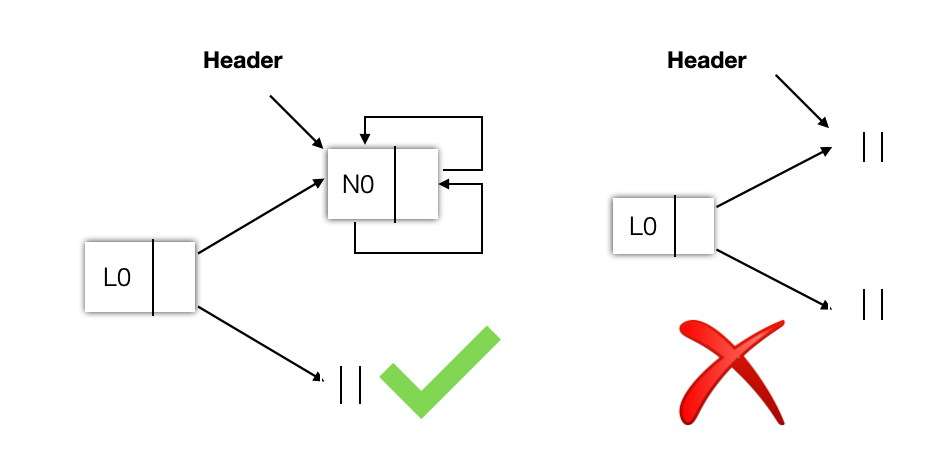
\includegraphics[width=0.8\textwidth]{images/repOK1.jpg}
        \caption{Ejemplo de una instancia válida y otra no válida de acuerdo al \emph{repOK} en la estructura general.}
        \label{fig:repOKa}
    \end{subfigure}

    \vspace{10pt}

    \begin{subfigure}[b]{\textwidth}
        \centering
        \includegraphics[width=0.8\textwidth]{images/repOK2.jpg}
        \caption{Ejemplo de una instancia válida y otra no válida de acuerdo al \emph{repOK} en la lista principal.}
        \label{fig:repOKb}
    \end{subfigure}

    \vspace{10pt}

    \begin{subfigure}[b]{\textwidth}
        \centering
        \includegraphics[width=0.8\textwidth]{images/repOK3.jpg}
        \caption{Ejemplo de una instancia válida y otra no válida de acuerdo al \emph{repOK} en la lista caché.}
        \label{fig:repOKc}
    \end{subfigure}

    \caption{Ejemplos de instancias de \texttt{NodeCachingLinkedList}.}
    \label{fig:repOK}
\end{figure}


En la Figura~\ref{fig:repOK} se muestran ejemplos de instancias válidas e inválidas, lo cual facilita entender visualmente las propiedades que deben estar reflejadas en la especificación.

Las líneas 2 a 10 del método se centran en la verificación de aspectos estructurales básicos. Se asegura la existencia del 
nodo ficticio, que debe contener valor \texttt{null} y estar correctamente conectado. Su presencia facilita el manejo de 
la lista, actuando como ancla para los elementos reales. 
La parte superior de la Figura~\ref{fig:repOKa} representa la lista principal, mientras que la inferior muestra la caché. 
En el ejemplo, la instancia de la izquierda es válida; la de la derecha es inválida al no incluir un nodo ficticio, lo cual es detectado por las condiciones de las líneas 5 y 6.


Las líneas 11 a 20 validan que la lista principal sea circular y doblemente enlazada. Esto implica que el recorrido a partir 
del nodo ficticio se debe eventualmente volver a él, y que cada nodo debe tener enlaces consistentes hacia su anterior y su 
siguiente. En otras palabras, si avanzamos a través de la lista desde el primer elemento, llegaremos eventualmente al
último elemento y luego volveremos al primer elemento. Además, se asegura que la cantidad de nodos visitados coincida con el valor del campo \texttt{size}.

En la Figura~\ref{fig:repOKb} se pueden observar ejemplos de instancias que satisfacen o no esta sección de restricciones del método.  
La instancia de la izquierda muestra una lista principal correctamente construida, mientras que la instancia de la derecha presenta el error de que la lista principal no es circular,  
una propiedad estructural que deben cumplir las listas principales (donde se almacenan los datos) en \texttt{NCL}.  
En esta instancia, el campo \emph{next} del nodo final no apunta nuevamente al nodo ficticio, lo que rompe la propiedad de circularidad de la estructura.  
Esta restricción está controlada en la línea 16 del método \texttt{repOK}.

Por su parte, las líneas 21 en adelante analizan la estructura de la caché, que debe ser una lista simple, acíclica, con nodos 
que no contengan valores. También se verifica que no haya nodos repetidos en la caché, y que la 
cantidad de elementos coincida con el valor de \texttt{cacheSize}.
Como ejemplo de esta situación, mostramos dos nuevas instancias en la Figura \ref{fig:repOKc}. 
La primera es una instancia válida de la lista caché y el \emph{repOK} nos devuelve \texttt{true}. 
La segunda instancia en la figura nos muestra una instancia inválida de acuerdo a la especificación. 
Esto se debe a que la lista caché (la lista de la parte inferior de la estructura) es cíclica. 
La insatisfacción de la propiedad se da cuando el método vuelve a insertar el mismo nodo al conjunto \emph{visited}. 
Este conjunto recorre la lista y chequea en la línea 31 si vuelve a pasar por un nodo ya visitado. 
En caso de que esto suceda, retorna \texttt{false}. 

Este ejemplo permite evidenciar que incluso estructuras relativamente simples requieren de especificaciones formales 
detalladas y cuidadosas. La ausencia o incorrecta implementación de restricciones puede resultar en la 
generación de instancias que no representan adecuadamente el dominio, afectando negativamente la efectividad de los 
procesos de verificación y prueba.


Este método \emph{repOK} está implementado siguiendo las recomendaciones de los
autores del enfoque de generación exhaustiva acotada de \textsf{Korat} \cite{Boyapati02}. 
La función devuelve \emph{falso} tan pronto como detecta una violación en alguna propiedad esperada de la estructura actual. 
En caso contrario, devuelve \emph{verdadero} al finalizar el método. 
Este enfoque permite a \textsf{Korat} podar eficientemente grandes porciones del espacio de búsqueda al encontrar restricciones incumplidas, mejorando así significativamente su eficiencia.

Sin embargo, en el \emph{repOK} que se presenta en la figura \ref{fig:NCL-repOK}, 
se puede observar que algunas restricciones están comentadas, 
lo que indica la ausencia de validaciones cruciales. 
Estas restricciones no estaban presentes en la versión original del \emph{repOK} que tomamos de Roops; 
las incorporamos después de analizar las estructuras generadas para las pruebas que resultaron incorrectas.

La omisión de restricciones en el \emph{repOK} tiene un impacto directo y considerable en la cantidad de estructuras que \textsf{Korat} genera. 
Esta falta de precisión no solo aumenta exponencialmente el número de estructuras generadas, 
sino que también complica la tarea de identificar cuáles son válidas y cuáles no. 
Por ejemplo, cuando se ejecuta \textsf{Korat} con el \emph{repOK} sin las restricciones comentadas, 
se generan 54.5 millones de estructuras para un \emph{scope} de 8. Al incluir las restricciones faltantes, 
la cantidad de estructuras generadas se reduce drásticamente a solo 2.8 millones para el mismo \emph{scope}.

Este incremento masivo en la generación de estructuras debido a la omisión de restricciones tiene implicaciones graves para el proceso de testing. 
Aumenta la probabilidad de que se generen falsos positivos, es decir, estructuras que cumplen con las propiedades básicas pero que no son representativas de casos válidos. 
Estos falsos positivos pueden llevar a realizar pruebas innecesarias o a interpretar incorrectamente los resultados del testing, comprometiendo la calidad del software.

Motivados por estos desafíos y la complejidad inherente a la escritura de métodos \emph{repOK} precisos para la generación exhaustiva acotada, hemos desarrollado una técnica que hemos denominado BEAPI. 
Esta técnica será detallada en las siguientes secciones, y busca ofrecer una solución más robusta y precisa para la generación y validación de estructuras en el contexto de pruebas exhaustivas.

\section[BEAPI]{BEAPI}
\label{sec:beapiIntro}
\cacho{Es nuevo esto:}
En esta sección discutimos las ideas principales de nuestros enfoques para generar de manera eficiente un conjunto exhaustivo acotado de objetos, haciendo solo llamadas a la API de un módulo. Nuestro enfoque se basan en la generación de pruebas dirigida por retroalimentación, explicado en la sección \ref{sec:feedback-directed-test-gen}.
El enfoque propuesto, denominado \textsf{BEAPI} (Bounded Exhaustive from an API), introduce una técnica innovadora para la generación exhaustiva acotada. Este enfoque se basa en la realización de llamadas a los métodos de la API del software bajo prueba (SUT). Al igual que otros enfoques de generación de pruebas basados en API, \textsf{BEAPI} crea secuencias de llamadas a métodos de la API, conocidas como secuencias de test \cite{Ammann16}, y las ejecuta para generar estructuras. 

\section{Visión general de BEAPI}
\label{sec:beapi-overview}

\begin{figure}[H]
  \centering
  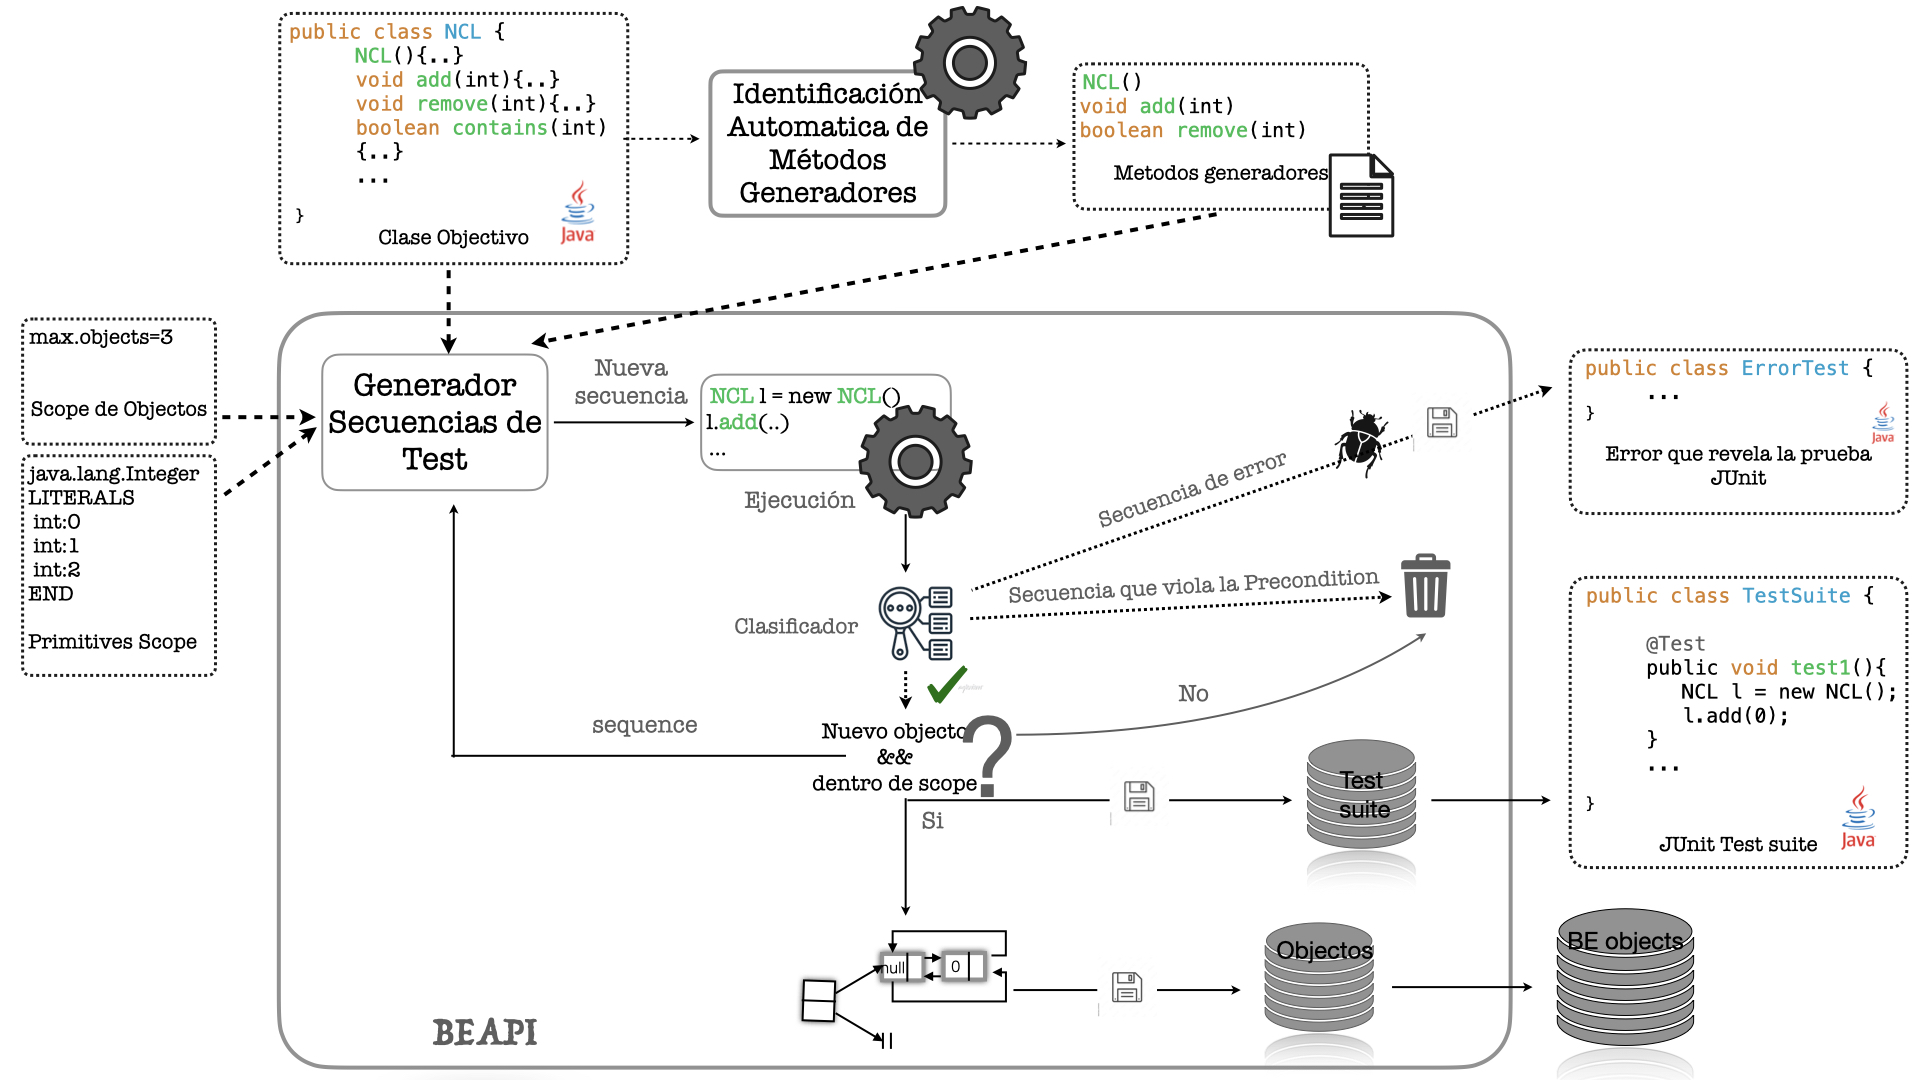
\includegraphics[width=1.0\textwidth]{images/beapi-arquitecture.jpeg}
  \caption{Arquitectura general de \textsf{BEAPI}}
  \label{fig:beapi-overview}
\end{figure}


La Figura~\ref{fig:beapi-overview} muestra una visión general de la herramienta 
\textsf{BEAPI} (\emph{Bounded Exhaustive from an API}), que implementa un enfoque 
de generación exhaustiva acotada de objetos mediante llamadas exclusivamente a 
la API de un módulo. 

Este enfoque se basa en la generación de pruebas dirigida por retroalimentación 
(\emph{feedback-directed test generation}, ver Sección~\ref{sec:feedback-directed-test-gen}). 
Al igual que otros enfoques de generación de pruebas basados en API, 
\textsf{BEAPI} construye secuencias de llamadas a métodos de la API 
(\emph{test sequences}~\cite{Ammann16}) y las ejecuta para producir estructuras.

\textsf{BEAPI} aborda las dificultades de escribir especificaciones formales 
para la generación exhaustiva acotada aprovechando la ejecución directa de las 
rutinas de la API y aplicando técnicas de poda para mejorar la eficiencia y 
permitir la escalabilidad a alcances mayores.

% Entradas y salidas
Como entradas, \textsf{BEAPI} recibe:
\begin{itemize}
    \item la clase o clases objetivo para la generación de casos de prueba;
    \item archivos de configuración que definen los límites de scope y los valores primitivos que se usaran para la generación;
    \item un archivo con los métodos de la clase objetivo que se emplearán 
    como \emph{métodos generadores de objetos}.
\end{itemize}

Como salidas, \textsf{BEAPI} produce:
\begin{itemize}
    \item un conjunto acotado y exhaustivo de objetos generados;
    \item una suite de pruebas \texttt{JUnit}~\cite{junit} con las secuencias 
    utilizadas para generar cada objeto;
    \item otra suite con secuencias que revelan errores en los métodos utilizados 
    para la generación.
\end{itemize}

% Flujo general de generación
El módulo \emph{generador de secuencias de test} (Figura~\ref{fig:beapi-overview}) 
comienza creando todas las secuencias de longitud~1 (una única invocación).  
Los valores primitivos definidos en la configuración se usan para instanciar 
parámetros.  

Cada secuencia se ejecuta, y aquellas que generan nuevos objetos (diferentes 
a los ya obtenidos) se retroalimentan al generador. A partir de ellas se 
construyen secuencias de longitud~2, y así sucesivamente.  

El proceso se repite hasta que las secuencias de longitud $k$ no generan nuevos 
objetos dentro del alcance definido por los \emph{scopes}. En ese momento, 
\textsf{BEAPI} detiene la generación y devuelve la suite y el conjunto de 
objetos.

% Clasificación de resultados
El módulo \emph{clasificador} observa el resultado de cada ejecución y clasifica 
la secuencia en una de cuatro categorías:
\begin{enumerate}
    \item revela un error en algún método;
    \item viola una precondición de un método;
    \item genera un objeto fuera de alcance o repetido;
    \item genera al menos un nuevo objeto válido dentro del alcance.
\end{enumerate}

Los casos (3) y (4) corresponden a ejecuciones sin excepciones.  
Los objetos generados se \emph{canonizan}~\cite{Politano20} y se comprueba 
si ya existían o exceden el alcance. En caso afirmativo (3), la secuencia se 
descarta; si al menos un objeto es nuevo (4), se retroalimenta al generador 
y se almacena como prueba válida.

Los casos (1) y (2) corresponden a ejecuciones con excepciones.  
Siguiendo a Randoop~\cite{Pacheco07}, por defecto \textsf{BEAPI} interpreta 
\texttt{IllegalArgumentException} e \texttt{IllegalStateException} como 
violaciones de precondición (caso 2), y el resto como errores (caso 1).  
Este comportamiento es configurable.
La generación exhaustiva de todas las secuencias de prueba factibles a partir de rutinas hasta una longitud máxima, 
también conocida como generación por fuerza bruta, es un enfoque intrínsecamente combinatorio que consume una gran cantidad de recursos computacionales, 
incluso para alcances pequeños. 
Por lo tanto, \textsf{BEAPI} utiliza varias técnicas de poda que son fundamentales para mejorar su eficiencia y permitir la escalabilidad a alcances más grandes.
Estas optimizaciones son:

\begin{enumerate}
    \item \textbf{Limitación por alcance, (\emph{scope})} \textsf{BEAPI} restringe
      la generación de secuencias de prueba a combinaciones de objetos y valores primitivos
      definidos por un alcance máximo (\emph{scope}) configurado por el usuario. 
      Este alcance limita, por ejemplo, la cantidad máxima de objetos por clase, 
      los rangos para tipos numéricos y las cadenas de texto permitidas 
      (ver Sección~\ref{sec:scope}). De esta forma se reduce drásticamente 
      el espacio de búsqueda inicial.
    \item \textbf{Filtrado por excepciones:} \textsf{BEAPI} ejecuta las secuencias de prueba y descarta
      aquellas que producen excepciones que violan las reglas de uso de la API, como
      \emph{IllegalArgumentException} e \emph{IllegalStateException} en Java.
      (\emph{defensive programming}~\cite{Liskov00}, ver Sección~\ref{sec:defensiveProgramming})
    \item \textbf{Coincidencia de estados:} descarta secuencias de métodos que generan estructuras que ya han sido creadas por 
      secuencias de métodos exploradas previamente. Esta técnica se describe en detalle en la sección \ref{sec:stateMatching}.
    \item \textbf{Selección de métodos generadores:} utiliza un subconjunto 
      de métodos de la API identificado mediante un algoritmo \emph{greedy} y 
      una función de valoración para maximizar la cantidad de objetos generados 
      en el menor tiempo (Capítulo~\ref{cap:builders}).
\end{enumerate}

Con las optimizaciones deshabilitadas, \textsf{BEAPI} solo es práctico para 
alcances pequeños (e.g., tamaño 3)~\cite{Politano20}. Con ellas habilitadas, 
su rendimiento es comparable al de \textsf{Korat} (Capítulo~\ref{cap:experimental}).





% \pp{Esto no va acá. Va en una sección que se llama programación defensiva que
%     puede estar después de scope, y que se encarga de explicar esto, y cómo ejecutando un test
% se puede descartar una secuencia.}
% A diferencia de los enfoques de generación basados en caja negra, \textsf{BEAPI} no requiere una especificación formal de las propiedades de las estructuras. Al igual que otras técnicas de generación exhaustiva acotada (BEG), el usuario solo debe proporcionar los alcances para la generación, que se abordan en detalle en la sección correspondiente.  Esto permite generar estructuras válidas sin requerir una especificación detallada de las propiedades de las estructuras, reduciendo así la carga de trabajo para el programador.

% La principal ventaja de \textsf{BEAPI} es que requiere un esfuerzo menor de especificación para realizar la generación exhaustiva acotada. Si los métodos de la API utilizados en la generación son correctos, todas las estructuras generadas serán válidas para su construcción. El programador solo necesita asegurarse de que los métodos de la API lancen excepciones cuando se violen las reglas de uso, siguiendo un estilo de programación defensivo \cite{Liskov00}. En la mayoría de los casos, esto implica verificar condiciones muy simples en las entradas. Por ejemplo, el método para eliminar (\emph{remove(int)}) un elemento de una \texttt{NCL} en un índice pasado como parámetro lanza una \texttt{IllegalArgumentException} cuando se llama con un índice menor a 0 o mayor al \emph{size} de la lista. El \emph{listing} de la figura \ref{fig:algoProgDefensiva}  se puede observar que la implementación del método se encarga de cumplir con la especificación indicada \texttt{NCL}.
% Para hacer esto


A continuación, explicaremos en detalle cada una de estas optimizaciones.

\subsection{Scope}
\label{sec:scope}



En el contexto de la generación exhaustiva acotada, el término \emph{scope} se refiere al límite o alcance que se establece para la generación de estructuras. 
Es una restricción que define cuántos objetos de un tipo particular pueden aparecer en las estructuras generadas. 
Esta restricción es esencial para controlar el tamaño y la complejidad del espacio de búsqueda de estructuras durante 
la generación exhaustiva. Sin un límite en el número de objetos que pueden aparecer en las estructuras generadas,
 el espacio de búsqueda podría ser infinito o extremadamente grande. Esto hace que la generación sea impracticable en la mayoría de los casos debido al tiempo 
 y los recursos requeridos.  En muchos casos, el conjunto de estructuras relevantes o interesantes es finito y puede definirse mediante un \emph{scope} adecuado.
 Al generar solo un conjunto finito de estructuras, se pueden abordar de manera exhaustiva todos los casos posibles.

Para limitar el número de estructuras generadas, BEAPI necesita definirlo en un archivo de descripción simple en formato \texttt{java.properties}, 
en el cual, además, se establecen algunos otros parámetros. En la figura \ref{fig:NCL-fin-BEAPI}, en la línea 1, se puede observar como establecer 
el \emph{scope} para un caso específico con la sentencia \emph{max.objects}. Este valor (\emph{k}) debe ser un valor entero. Supongamos el caso de 
la figura \ref{fig:ncl-instances} de instancias de \texttt{NCL}.  El límite $k$ representa el número máximo de objetos que se pueden crear para cada 
clase (en la Figura \ref{fig:ncl-instances}, el número de nodos en los objetos NCL está acotado por $k=2$). Esto especifica el número máximo de objetos 
diferentes (alcanzables desde la raíz) permitidos en una estructura. Las secuencias de prueba generadas por \emph{BEAPI} que crean estructuras que 
exceden este número (para cualquier clase) se descartan y no se siguen extendiendo

\begin{figure}[H]
    \centering
    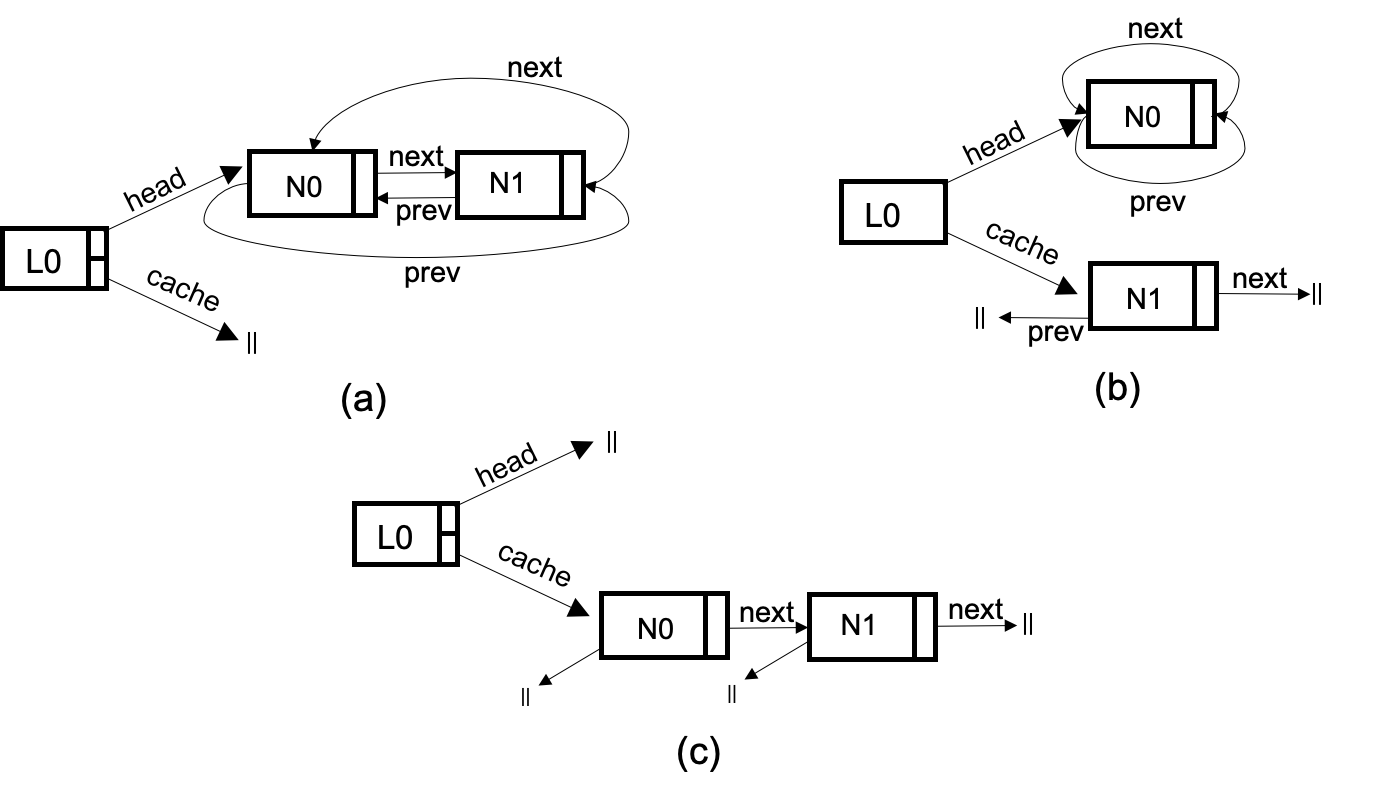
\includegraphics[width=0.85\textwidth]{images/NCL-instances.png}
    \caption{Tres instancias de NodeCachingLinkedList con exactamente dos nodos}
    \label{fig:ncl-instances}
\end{figure}
\pp{Esta figura es igual a la Figura 2? Digo porque hay otra con instancias
antes? Si la vamos a repetir en este capítulo capaz que convenga ponerla antes y
eliminar la otra?}

\begin{figure}[H]
\begin{lstlisting}[keywordstyle=\scriptsize\ttfamily]
max.objects=k
int.range=0:3
strings=str1,str2,str3
omit.fields=NCL.DEFAULT_MAXIMUM_CACHE_SIZE
\end{lstlisting}
\caption{Definición del scope de BEAPI para NCL (nodos max. 3)}
\label{fig:NCL-fin-BEAPI}
\end{figure}


Nuestra técnica, basada en generación de test por feedback, necesita, también, un conjunto de valores primitivos especificado por el usuario 
(enteros, strings, etc) que son utilizados para alimentar a los métodos (que requieran valores primitivos) de la API que se combinan para generar 
las estructuras del SUT que estamos buscando.
Por ejemplo, en la figura \ref{fig:scope} el método \emph{add(int)}, que agrega un elemento a la lista principal, 
necesita un entero para el campo \emph{value} de cada nodo. Este valor entero, como es un valor primitivo, 
se toma de algunos de los valores primitivos que definió el usuario en el archivo de configuración de BEAPI (\ref{fig:NCL-fin-BEAPI}). 
En la línea 2 y 3 se puede observar que define valores de tipo enteros y valores de tipo string que serán utilizados por los métodos 
cuando necesiten valores de este tipo. 
\\


\begin{figure}[H]
    \centering
    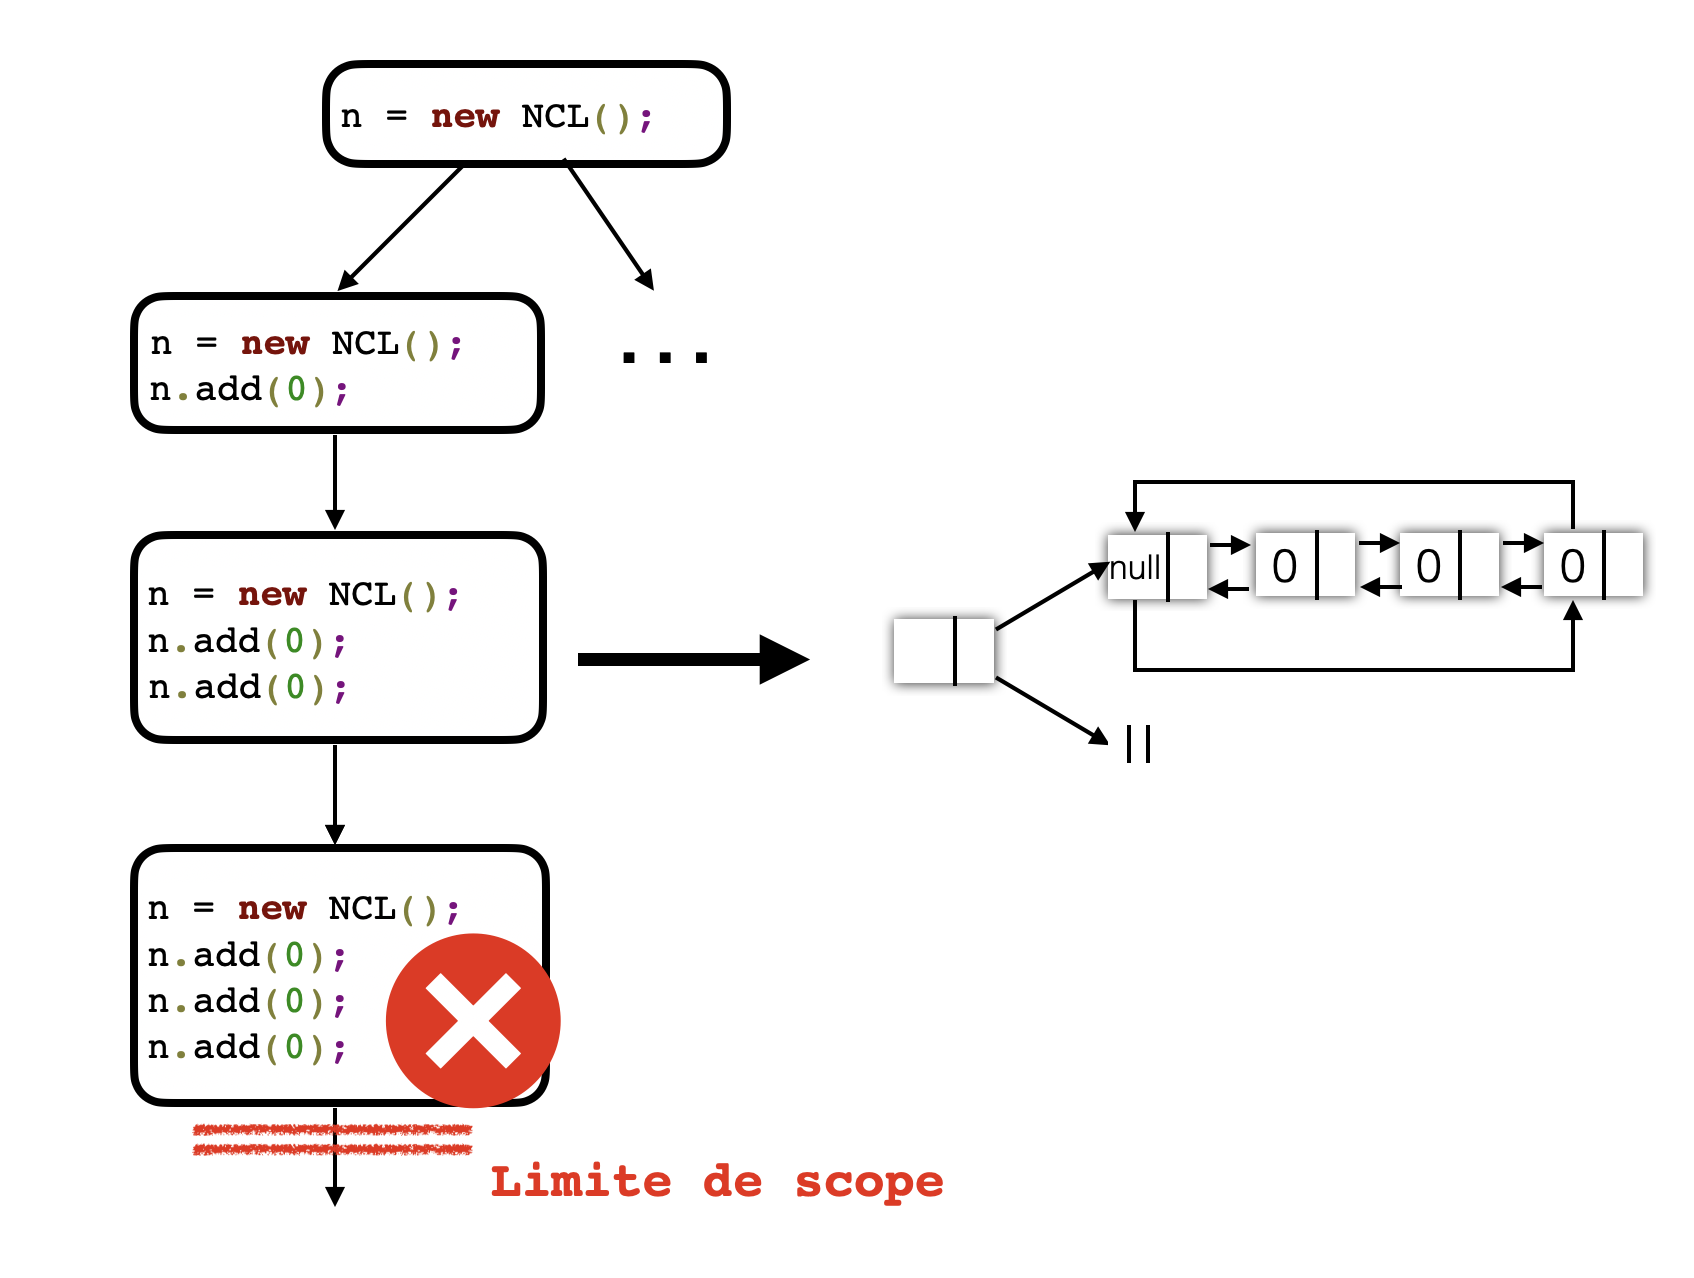
\includegraphics[width=0.85\textwidth]{images/scope.jpg}
    \caption{Representación con scope 3 para NCL}
    \label{fig:scope}
\end{figure}

\cacho{Explicar sobre objects que son int para nosotros? o
esconderlo?}\pp{Que algunos parámetros Object los interpretamos como int?
No sé si vale la pena meterse con eso, porque es sólo para casos específicos
donde la genericidad usa object, que no son muy comunes creo. Lo charlamos.}

Cómo último, nuestro archivo de configuración, permite que el usuario especifique que valores desea que no sean tenidos en cuenta a la hora de comparar estructuras. 
Esto toma especial importancia el contexto de estructuras de datos, especialmente en colecciones y contenedores en Java. En estos casos suelen aparecer campos en la clase que representa un contador de modificaciones o cambios realizados en la estructura de datos. Comúnmente son llamados \emph{modCount}. 
Este es un campo que se utiliza para realizar un seguimiento de las modificaciones que se han realizado en la colección desde su creación o desde la última vez que se realizó un seguimiento. 
El \emph{modCount} es un campo de tipo entero que se incrementa cada vez que se realiza una modificación en la estructura de datos. Las modificaciones pueden incluir inserciones, eliminaciones, actualizaciones u otras operaciones que afecten la colección. 
El propósito principal de llevar un contador de modificaciones es facilitar la detección de modificaciones concurrentes o cambios inesperados en la colección por parte de múltiples hilos de ejecución. 
En la línea 4 del archivo de configuración \ref{fig:NCL-fin-BEAPI}, se puede observar como se especifica aquellos campos que deseamos omitir a la hora de tener una representación canónica de la estructura. Canonicalizar un objeto se refiere a la acción de garantizar que un objeto se encuentre en su forma más básica y representativa, lo que facilita las comparaciones y operaciones con otros objetos similares.
Para lograr todo lo explicado en esta sección, nosotros canonizamos los objetos generados por la ejecución de cada secuencia de métodos y analizamos y trabajamos con su representación canónica.
Para finalizar esta sección, se puede observar en la figura \ref{sec:scope} un ejemplo del espacio de búsqueda de una secuencia generada con la combinación del método constructor de la clase más el método \emph{add} de NCL. En esta figura, se especificó un scope de 3. Esto quiere decir que cuando genera alguna estructura con más de 3 nodos como es en el caso de la última secuencia de la figura, esta es descartada por exceder el límite de nodos en la estructura (el nodo ficticio de la estructura se tiene en cuenta en la definición de \emph{scope})

% \pp{Esta canonización no coincide con la que se explica en state matching, que
%     implica recorrer un grafo y generar una secuencia. Yo no sé si pondría este
% ejemplo. De cualquier modo, no va acá en la sección de scope, de última va para
% state matching. Yo cerraría la sección acá.}
% Imaginemos un conjunto de números representado en diferentes órdenes:
% \begin{itemize}
%     \item Conjunto 1: \{3, 1, 2\}
%     \item Conjunto 2: \{1, 2, 3\}
%     \item Conjunto 3: \{2, 3, 1\}
% \end{itemize}

% Aunque los elementos de cada conjunto son los mismos, el orden de los números varía. Si quisiéramos comparar estos conjuntos para determinar si son equivalentes, el proceso de canonización podría consistir en ordenar los números en cada conjunto de manera ascendente:

% \begin{itemize}
%     \item Conjunto 1 canonizado: {1, 2, 3}
%     \item Conjunto 2 canonizado: {1, 2, 3}
%     \item Conjunto 3 canonizado: {1, 2, 3}
% \end{itemize}

% Tras la canonización, todas las versiones del conjunto resultan idénticas, lo que nos permite determinar fácilmente que los tres conjuntos son equivalentes, independientemente del orden en el que aparecían originalmente los números.

% En el contexto de estructuras de datos, este proceso podría implicar reorganizar los nodos, normalizar los valores de ciertos campos, o eliminar detalles que no son relevantes para la comparación, como el \emph{modCount} mencionado anteriormente. Al canonizar, se asegura que dos estructuras de datos se comparen en términos de su contenido esencial, ignorando diferencias superficiales o de implementación.

% (Normalmente, las técnicas basada en generación por retroalimentación guardaría los valores primitivos que son devueltos por la ejecución de las pruebas y reutilizaría estos valores en pruebas futuras). 
% También nuestra técnica descartar secuencias de métodos que crean objetos con más de $k$ objetos (de cualquier tipo), para evitar que se construyan objetos más grandes de lo necesario. 


% \cacho{VER BIEN ESTO DE NO EXTENDERSE, porq para crear estrucutras de 3 nodos a veces necesito crear previamente una de 4 nodos}
% Esto asegura que se generen solo \texttt{NCL} con no más de k nodos. 
% Por ejemplo, la figura \ref{fig:scope}, se puede observar que cuando genera una estructura con mas nodos que el especificado en el archivo de configuración, 
% este no sigue extiendo el árbol de búsqueda. En la figura el scope especificado es 3 (vale aclarar, que el nodo ficticio cuanta como nodo de la estructura.)


% Siguiendo el análisis del archivo de configuración de la figura \ref{fig:NCL-fin-BEAPI},
% y el número de valores primitivos disponibles, en nuestro ejemplo de la figura, se especifica enteros del 0 a $k-1$ y cadenas de caracteres: str1, str2, str3. Ademas, se pueden especificar otros valores primitivos como floats, doubles, etc. Esto serán los dominios de datos para los tipos primitivos que necesiten los métodos que serán utilizados. Podemos indicarle a \emph{BEAPI} que ignore algunos campos en el proceso de canonización de objetos, que se lleva a cabo en la ejecución de las secuencias de métodos de la API. Esto permite al usuario controlar qué partes de la estructura del objeto son relevantes para la coincidencia de estados (ver más adelante en la sección \ref{sec:stateMatching}). Por ejemplo,  la línea 4 haría que \emph{BEAPI} omita el tamaño máximo predeterminado de la caché en la coincidencia de estados, que en la API de \emph{NCL} es una constante inicializada en 20 en el constructor de la clase. Es importante que aquí se omitan campos que puede afectar la coincidencia de estados, como el caso del campo \emph{modCount}. Esta variable se utiliza a menudo en estructuras de datos para realizar un seguimiento de las modificaciones o cambios realizados en los datos almacenados, pero claramente no afecta la estructura generada. 
% La configuración mostrada en la Figura~\ref{fig:NCL-fin-BEAPI} es suficiente para que \emph{BEAPI} genere NCL con un máximo de 3 nodos, que contienen enteros del 0 al 2 como valores. 

\subsection{Programación Defensiva}
\label{sec:defensiveProgramming}

\cacho{Toda esta seccion es nueva, solo un parrafo ya estaba.}
Una de las principales ventajas del enfoque \textsf{BEAPI} frente a otras técnicas de generación automática de estructuras 
es que no requiere de una especificación formal explícita para restringir el espacio de búsqueda. 
En lugar de depender de invariantes de representación complejos, como ocurre en técnicas basadas en generación exhaustiva acotada tradicional 
(e.g., \textsf{Korat}), \textsf{BEAPI} se apoya en la definición de métodos correctos provistos por la API de la clase bajo prueba.

Esto es posible gracias a la adopción de un estilo de \emph{programación defensiva}~\cite{Liskov00} en el diseño de estos métodos. 
La programación defensiva es una técnica que promueve la validación de precondiciones en los métodos públicos, de modo que los errores 
relacionados con el uso incorrecto de la API puedan ser detectados y reportados mediante excepciones apropiadas.

En el contexto de \textsf{BEAPI}, esta práctica permite descartar automáticamente secuencias de métodos que violan las restricciones de uso 
de la clase, ya que los tests generados que invocan métodos con parámetros inválidos o en estados inconsistentes provocan una excepción 
durante la ejecución. Dado que \textsf{BEAPI} ejecuta cada secuencia como parte del proceso de exploración, este mecanismo actúa 
como un filtro dinámico: las secuencias inválidas no se consideran como candidatas válidas para generar nuevas estructuras.

\begin{figure}[!htb]
\begin{lstlisting}
public Object removeIndex(int index) {
  // Verificacion de precondicion
  if(index < 0 || index >= size)
      throw new IllegalArgumentException();  
   \dots
   }
\end{lstlisting}
\caption{Programación defensiva en un metodo en \texttt{NodeCachingLinkedList}.}
\label{fig:algoProgDefensiva}
\end{figure}

El código mostrado en la Figura~\ref{fig:algoProgDefensiva} ejemplifica esta técnica. 
El método \texttt{removeIndex} de la clase \texttt{NodeCachingLinkedList} verifica que el índice especificado se encuentre dentro de los límites válidos de la lista. 
Si la condición no se cumple, se lanza una excepción que permite a \textsf{BEAPI} descartar automáticamente la secuencia correspondiente 
sin necesidad de especificar esta restricción en un invariante externo.

Este enfoque reduce significativamente la carga de trabajo del usuario, ya que no es necesario escribir un \texttt{repOK} manual ni mantenerlo 
en sincronía con la implementación. En cambio, basta con asegurar que los métodos de la API respeten buenas prácticas de validación 
de entradas y mantengan la clase en un estado consistente. 
De este modo, \textsf{BEAPI} puede aprovechar la ejecución dinámica de los tests para delimitar correctamente el espacio de estructuras válidas.


\subsection{State Matching}
\label{sec:stateMatching}
\cacho{Explique un poco mejor la parte de la figura, no me parece agregar mucho mas al respecto. Lo podemos charlar}
Durante la generación exhaustiva de secuencias de prueba, pueden surgir múltiples caminos que conducen al mismo estado final. 
Estas secuencias redundantes aumentan innecesariamente el espacio de exploración, consumiendo recursos y tiempo de ejecución. 
Para mitigar este problema, \textsf{BEAPI} implementa una estrategia de coincidencia de estado(\emph{state matching} en inglés) que permite identificar y descartar caminos que conducen a estados ya generados.

Por ejemplo, crear una lista vacía, agregar un elemento, eliminarlo y luego volver a agregarlo, resulta en el mismo estado que simplemente agregar ese elemento a una lista vacía. 
De manera similar, intentar eliminar un elemento de una lista vacía no altera su estado, produciendo el mismo resultado que una lista recién creada. 
En estructuras como pilas, realizar una operación de \texttt{push}, seguida de un \texttt{pop} y un nuevo \texttt{push} del mismo valor, 
produce una configuración indistinguible de aquella que resulta de realizar únicamente el último \texttt{push}. 

Este tipo de situaciones es capturado por la estrategia de \emph{state matching}, que consiste en mantener un registro de las estructuras generadas durante la exploración, y descartar cualquier nueva secuencia que produzca una estructura ya observada. 
\textsf{BEAPI} asume que las ejecuciones de los métodos de la API son deterministas, es decir, cualquier ejecución de un método con las mismas entradas produce siempre el mismo resultado. 
Por tanto, si una secuencia de prueba conduce a una estructura que ya ha sido generada por una secuencia anterior, no es necesario seguir extendiendo la nueva secuencia, 
ya se han explorado sus consecuencias a través de la primera.
Si almacenamos muchas secuencias de prueba para la misma estructura, todas estas secuencias tendrían que ser extendidas con nuevas rutinas en iteraciones posteriores de \textsf{BEAPI}, 
lo que resultaría tener que realizar un cómputo de las secuencias que sería innecesario ya que producen un estado que ya hemos computado y que hemos extendido.  

En la Figura~\ref{fig:stateMatching}, se puede observar de manera mas clara, la explosion de estados. 
Cada nodo del árbol representa una secuencia de llamadas a la API sobre una instancia de \texttt{NodeCachingLinkedList}. 
Las flechas indican la evolución de los estados al ejecutar nuevas operaciones. 
Las marcas de \emph{visited state} \cacho{SACO EL INGLES?} indican que el estado generado ya ha sido explorado anteriormente. 
Como puede observarse, múltiples caminos llevan a la misma estructura, y continuar su expansión sería innecesario.

\begin{figure}[H]
  \centering
  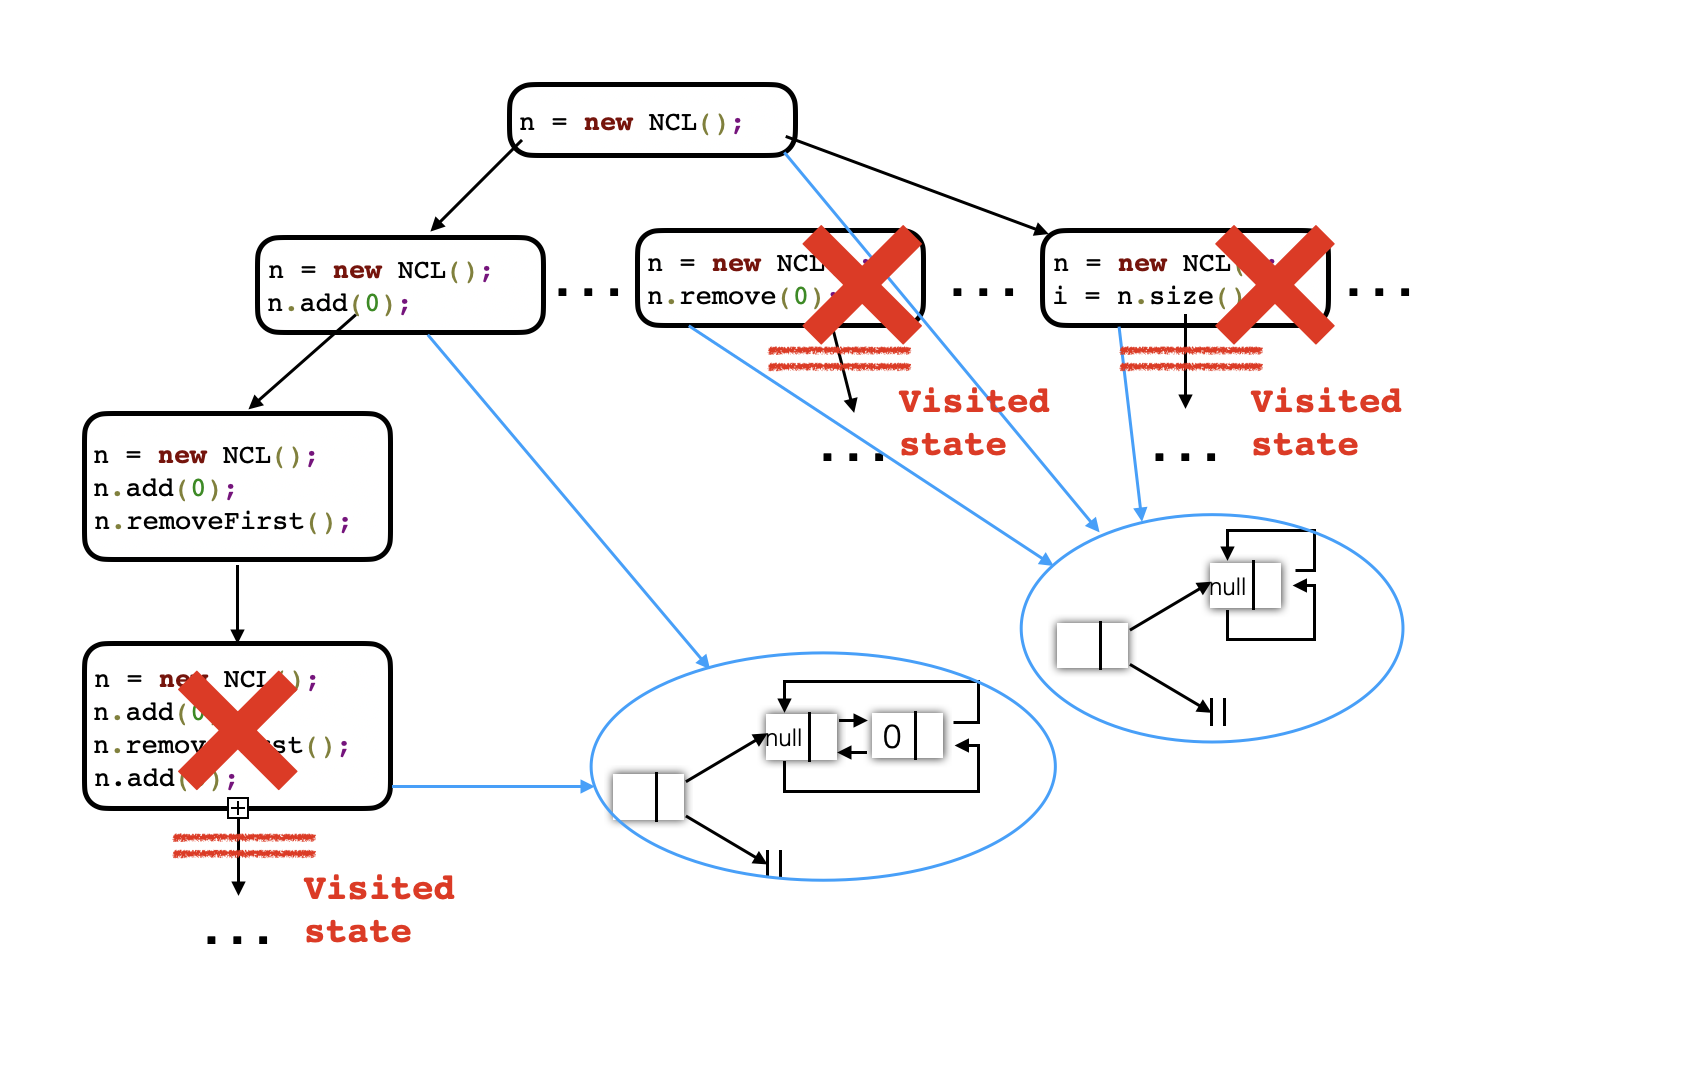
\includegraphics[width=1\textwidth]{images/stateMatching1.jpg}
  \caption{State matching en \emph{NodeCachingLinkedList}}
  \label{fig:stateMatching}
\end{figure}


\emph{State matching} es, por tanto, una optimización crítica para que la generación exhaustiva acotada pueda escalar a dominios con muchas combinaciones posibles de operaciones. 
Implementamos esta técnica en \textsf{BEAPI} mediante la transformación de las estructuras generadas a una representación canónica que permite su comparación eficiente.

Concretamente, \textsf{BEAPI} almacena todas las estructuras generadas hasta el momento en su forma canónica. 
Luego de ejecutar la última rutina \texttt{r(p$_1$, ..., p$_k$)} de una nueva secuencia de prueba \texttt{T}, 
el sistema verifica si alguno de los parámetros involucrados en \texttt{r} posee una estructura que no haya sido observada previamente (es decir, que no esté almacenada). 
Si ninguna estructura nueva es detectada, la secuencia \texttt{T} se considera redundante y es descartada. 
De lo contrario, \texttt{T} se almacena como secuencia representativa, junto con las nuevas estructuras producidas.

Representamos las estructuras asignadas en el heap como grafos etiquetados. 
Después de la ejecución de un método, un parámetro $p$ (de tipo no primitivo) 
contiene una referencia al objeto raíz $r$ de un \emph{heap} con raíz (es decir, $p=r$), definido a continuación.

\begin{definition}
Sea $O$ un conjunto de objetos y $P$ un conjunto de valores primitivos (incluido $null$). Sea $F$ el conjunto de campos de todos los objetos en $O$.
\begin{itemize}
\item Un \emph{heap} es un grafo etiquetado $H = \langle O, E\rangle$ con $E = {(o, f, v) | o \in O, f \in F, v \in O \cup P}$.
\item Un \emph{heap con raíz} es un par $RH = \langle r, H \rangle$ donde $r \in O$, $H = \langle O, E\rangle$ es un heap, y para cada $v' \in O \cup P$, $v'$ es alcanzable desde $r$ a través de campos en $F$.
\end{itemize}
\end{definition}

El caso especial $p = null$ se puede representar con un \emph{heap} con raíz que tiene un nodo ficticio y un campo ficticio que apunta a null. En lenguajes como Java, cada objeto se identifica por la dirección de memoria donde se encuentra. Cambiar las direcciones de memoria donde se asignan los objetos no tiene efecto desde el punto de vista del programa, ya que el programador no tiene control sobre la representación de bajo nivel de la memoria (a diferencia de otros lenguajes como C). Los \emph{heaps} obtenidos mediante permutaciones de las direcciones de memoria de sus objetos componentes se llaman \emph{heaps isomorfos}. Evitamos la generación de \emph{heaps isomorfos} empleando una representación canónica para los heaps \cite{Iosif02,Boyapati02}. Los heaps con raíz se pueden canonizar eficientemente mediante un enfoque llamado \emph{linearización} \cite{Iosif02,Xie04}, que transforma un heap con raíz en una secuencia única de valores.

\bigbreak

% \begin{figure}[!th]
% \begin{lstlisting}
% int[] linearizar(O raiz, Heap<O, E> heap, int alcance, Regex omitirCampos) {
%     Map ids = new Map(); // mapea nodos a sus identificadores unicos
%     return lin(raiz, heap, alcance, ids, omitirCampos);
% }
% int[] lin(O raiz, Heap<O, E> heap, int alcance, Map ids, Regex omitirCampos) {
%     if (ids.containsKey(raiz))
%         return secuenciaUnica(ids.get(raiz));
%     if (ids.size() == alcance)
%         throw new excepcionAlcanceSuperado();
%     int id = ids.size() + 1;
%     ids.put(raiz, id);
%     int[] seq = secuenciaUnica(id);
%     Edge[] campos =
%     ordenarPorCampo({ <raiz, f, o> en E }, omitirCampos);
%     foreach (<raiz, f, o> en campos) {
%         if (esPrimitivo(o))
%             seq.add(representacionUnica(o));
%         else
%             seq.append(lin(o, heap, alcance, ids, omitirCampos));
%     }
%     return seq;
% }
% \end{lstlisting}
% \caption{Algoritmo de linearización}
% \label{alg:linearization}
% \end{figure}

\cacho{Cambios minimos, sacado del paper de BEAPI, algoritmo en ingles en vez de español.}



\begin{figure}[!th]
\begin{lstlisting}
int[] linearize(O root, Heap<O, E> heap, int scope, Regex omitFields) {
    Map ids = new Map(); // maps nodes into their unique ids 
    return lin(root, heap, scope, ids, omitFields); 
}
int[] lin(O root, Heap<O, E> heap, int scope, Map ids, Regex omitFields) { 
  if (ids.containsKey(root))
    return singletonSequence(ids.get(root)); 
  if (ids.size() == scope) 
    throw new ScopeExceededException();
  int id = ids.size() + 1;
  ids.put(root, id);
  int[] seq = singletonSequence(id);
  Edge[] fields = sortByField({ <root, f, o> in E }, omitFields); 
  foreach (<root, f, o> in fields) {
    if (isPrimitive(o)) 
      seq.add(uniqueRepresentation(o));
    else
      seq.append(lin(o, heap, scope, ids, omitFields));
  }
  return seq; 
}
\end{lstlisting}
\caption{Algortirmo de linearización }
\label{alg:linearization}
\end{figure}
% java.util.LinkedList.MAX_ARRAY_SIZE&java.util.LinkedList:0&2147483639
% java.util.LinkedList.first&java.util.LinkedList:0&java.util.LinkedList$Node:0
% java.util.LinkedList.last&java.util.LinkedList:0&java.util.LinkedList$Node:1
% java.util.LinkedList.modCount&java.util.LinkedList:0&2
% java.util.LinkedList.serialVersionUID&java.util.LinkedList:0&876323262645176354
% java.util.LinkedList.size&java.util.LinkedList:0&2
% traversal.DummyHeapRoot.theroot&traversal.DummyHeapRoot:0&java.util.LinkedList:0


Figura\ref{alg:linearization} muestra el algoritmo de linealización utilizado por \textsf{BEAPI}, una versión personalizada que 
informa cuando los objetos exceden el \emph{scope} y permite ignorar ciertos campos de los objetos (para la versión original, véase 
\cite{Xie04}). El procedimiento \texttt{linearize} inicia un recorrido en profundidad del heap a partir de un objeto raíz, invocando 
\texttt{lin} en la línea 3. Para canonicizar el heap, \texttt{lin} asigna identificadores únicos a cada objeto que visita. El mapa 
\texttt{ids} almacena la correspondencia entre objetos y sus identificadores únicos.

Figure\ref{alg:linearization} muestra el algoritmo de linealización utilizado por \textsf{BEAPI}, una versión personalizada que 
informa cuando los objetos exceden el \emph{scope} y permite ignorar ciertos campos de los objetos (para la versión original, véase 
\cite{Xie04}). El procedimiento \texttt{linearize} inicia un recorrido en profundidad del heap a partir de un objeto raíz, invocando 
\texttt{lin} en la línea 3. Para canonicizar el heap, \texttt{lin} asigna identificadores únicos a cada objeto que visita. El mapa 
\texttt{ids} almacena la correspondencia entre objetos y sus identificadores únicos.

Cuando un objeto es visitado por primera vez, se le asigna un nuevo identificador (líneas 10--11), y se crea una secuencia \emph{singleton}
que representa dicho objeto (línea 12). A continuación, se recorren los campos del objeto, ordenados en un orden predefinido (por 
ejemplo, alfabéticamente por nombre), y se construye la linealización de cada valor de campo, concatenando el resultado a la secuencia 
del objeto actual (líneas 13--19). Si un campo contiene un valor primitivo, se lo representa mediante una secuencia singleton con dicho 
valor (líneas 15--16). Si un campo referencia a otro objeto, se realiza una llamada recursiva a \texttt{lin} para convertir dicho objeto 
en una secuencia, la cual se añade al resultado (línea 18). Al finalizar el bucle, \texttt{seq} contiene la representación canónica del 
heap con raíz en \texttt{root}, y se devuelve como resultado (línea 20).

Cuando un objeto ya visitado es alcanzado por una llamada recursiva, el mismo ya debe tener un identificador asignado en \texttt{ids} 
(línea 6), y \texttt{lin} retorna la secuencia singleton correspondiente (línea 7). Si durante el proceso se detecta que la cantidad de 
objetos alcanzables excede el \emph{scope} permitido, se lanza una excepción \texttt{ScopeExceededException} (líneas 9--10). Esta 
excepción será utilizada por \textsf{BEAPI} para descartar aquellas secuencias de prueba que generan objetos más grandes de lo 
permitido por el \emph{scope}.

El procedimiento \texttt{linearize} también recibe como parámetro una expresión regular \texttt{omitFields}, que define los nombres 
de los campos que deben ser ignorados durante la linealización. Para omitir estos 
campos, la función \texttt{sortByField} (línea 13) ha sido implementada de forma tal que no devuelve las aristas correspondientes a 
los campos cuyo nombre coincide con \texttt{omitFields}. Esto evita que los valores de dichos campos se incluyan en la secuencia 
resultante.

Finalmente, la linealización permite comparar estructuras de manera eficiente: dos objetos (es decir, dos heaps enraizados) son iguales 
si, y solo si, las secuencias generadas por \texttt{linearize} son iguales.

\subsection{Uso de m\'etodos generadores de objectos en BEAPI}
\label{sec:buildersOptimization}
En esta sección, utilizaremos una optimización que hemos desarrollado y que es
una parte importante de esta tesis (Capítulo \ref{cap:builders}.
Estos métodos generadores nos permiten generar cualquier configuración posible que se puede construir con la API (pudiendo generar de manera exhaustiva, es decir, generando todos los objetos posibles hasta un alcance dado).
Dado que la cantidad de combinaciones factibles de métodos crece de manera exponencial con el número de métodos,
es crucial reducir la cantidad de métodos que \textsf{BEAPI} utiliza para producir secuencias de prueba. Para abordar este problema, 
utilizamos el enfoque de identificación automática de métodos generadores que se describe en el Capítulo \ref{cap:builders}.
Este enfoque nos ayuda a encontrar un subconjunto de métodos de la API que son suficientes para generar conjuntos de estructuras acotadas y exhaustivas. 
El uso de métodos generadores permite generar estados complejos sin necesidad de ejecutar múltiples pasos individuales. Esto reduce significativamente la cantidad de secuencias que BEAPI necesita explorar, optimizando el análisis. 

En el contexto de \textsf{BEAPI}, utilizamos el algoritmo de búsqueda de tipo Greedy para identificar este subconjunto de métodos generadores.
El enfoque está basado en el algoritmo de optimización \emph{Escalada de colinas} que logra un mejor rendimiento. 
Aunque \emph{Escalada de colinas} puede ser menos preciso, ya que puede incluir algunos métodos que no son necesarios para producir un conjunto acotado y exhaustivo de estructuras, 
en nuestros experimentos, el algoritmo de \emph{escalada de colinas}  funcionó muy bien y calculó consistentemente conjuntos sufientes de métodos generadores (verificamos que coincidieran con los métodos que identificados manualmente y que son generadores en cada caso de estudio). 
% Nuestro objetivo aquí es evaluar el impacto de utilizar builders para la generación exhaustiva acotada (BEG) a partir de una API.

Para la identificación de métodos generadores, utilizamos como función de evaluación un generador exhaustivo para crear objetos de la API (ver sección \ref{sec:fitness}). 
Este generador es precisamente BEAPI que estamos desarrollando en esta sección. 
La idea clave que hace factible la identificación de los métodos generadores es que a menudo los generadores identificados para un \emph{scope} relativamente pequeño 
utilizan el mismo conjunto de métodos que se necesitan para crear estructuras de cualquier tamaño.
En otras palabras, una vez que el alcance para el cálculo de los métodos generadores es lo suficientemente grande, aumentar el alcance producirá como resultado el mismo conjunto de constructores. 
Este resultado se asemeja a la hipótesis de la cota pequeña para la detección de errores[\cite{Andoni02} (a la técnica de \emph{transcoping} \cite{Rosner13}).
En todos nuestros casos de estudio, un \emph{scope} de 5 fue suficiente para calcular los métodos generadores de objetos. 
Después de identificar eficientemente los métodos generadores con un alcance pequeño, podemos ejecutar \textsf{BEAPI}, utilizando los métodos generadores identificados y,
con un alcance mayor. Esto nos permite generar objetos más grandes y utilizarlos para probar el software bajo prueba.

En la mayoría de nuestros casos de estudio, los métodos generadores de objetos se limitan a un 
constructor y un único método para agregar elementos a la estructura, como ocurre en las listas 
simplemente enlazadas.  

Sin embargo, nuestro enfoque automatizado de identificación de métodos generadores evidenció que, 
en el caso de los árboles Rojo–Negro, también es necesario incluir un método de eliminación 
(para alcances mayores que tres).  
Esto se debe a que este tipo de árboles requiere configuraciones específicas de equilibrio, 
que involucran el coloreo de nodos en rojo y negro, las cuales no pueden obtenerse únicamente 
mediante operaciones de inserción.


En contraste, los árboles AVL,
que también son estructuras balanceadas, no requieren el método de eliminación como parte de su subconjunto de métodos generadores.
Los árboles AVL están siempre equilibrados, 
de tal modo que para todos los nodos, la altura de la rama izquierda no debe diferir en más de una unidad de la altura de la rama derecha o viceversa. 
Gracias a esta forma de equilibrio (o balanceo), la complejidad de una búsqueda en uno de estos árboles se mantiene siempre en orden de complejidad O(log n). 
Para este caso de árboles, solo el constructor de la clase y una rutina de adición son suficientes. 
Esto demuestra que la identificación de métodos generadores no es trivial de realizar manualmente.

\begin{figure}
  \centering
  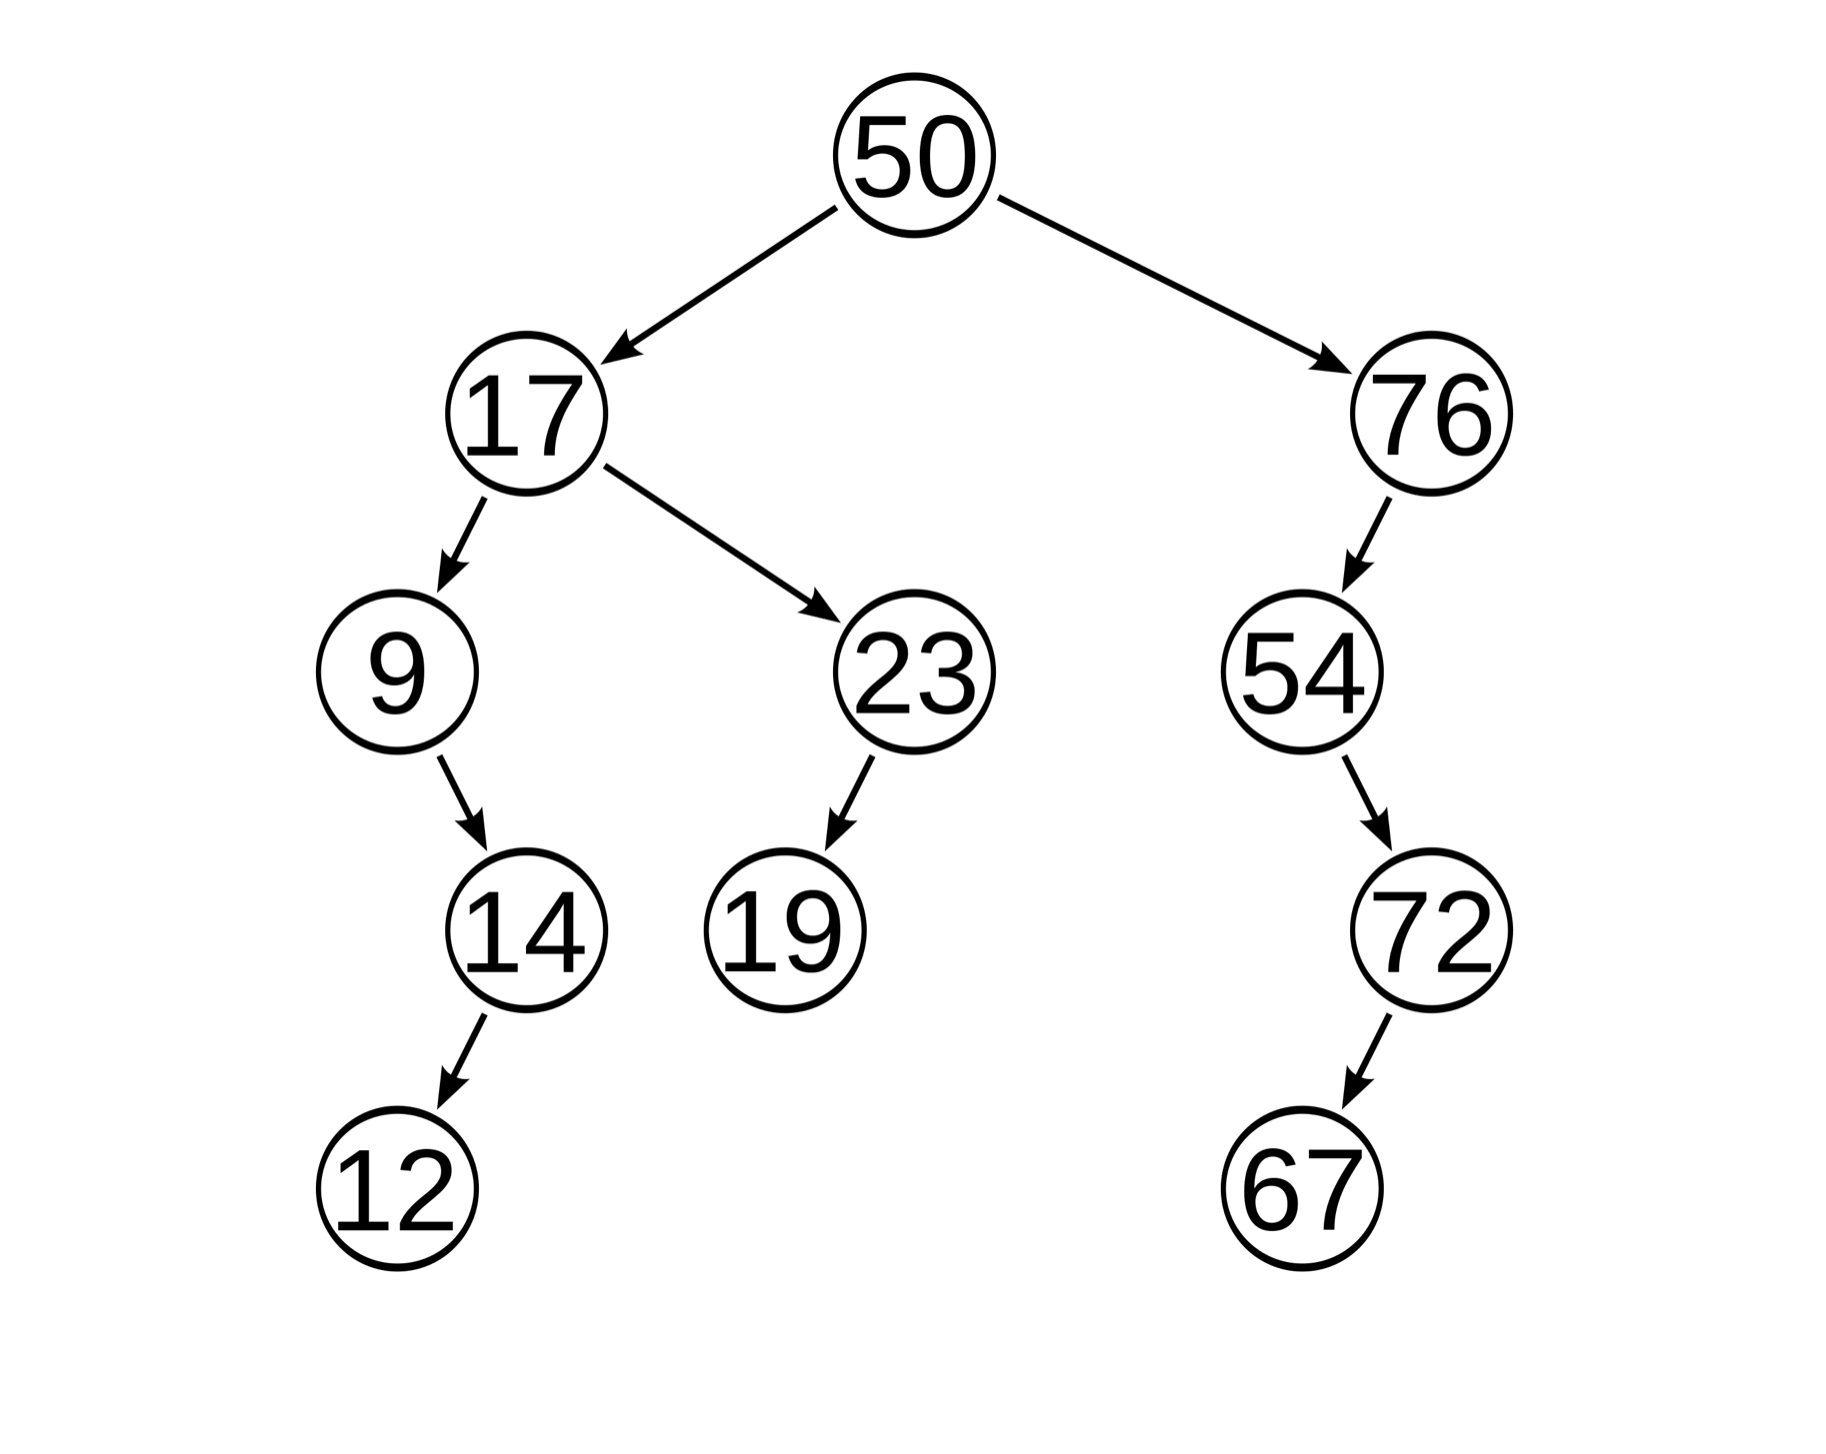
\includegraphics[width=0.7\textwidth]{images/avl.jpg}
  \caption{Ejemplo de un árbol AVL}
  \label{fig:avl}
\end{figure}

\section{Algoritmo de BEAPI}
\label{sec:beapiTechnique}

A continuación se muestra un pseudocódigo de \emph{BEAPI} en la Figura \ref{fig:beapi-algorithm}. 
\emph{BEAPI} toma como entradas una lista de métodos de una API,  \texttt{methods}. 
Estos métodos pueden ser la API completa o un subconjuntos de métodos de la misma. 
En nuestro caso, como hemos aplicado anteriormente, vamos a utilizar los métodos generadores previamente identificados. 
Además, el algoritmo recibe de parámetro, el alcance (\emph{scope}) de objetos para la generación; una lista para crear valores de cada tipo primitivo proporcionado en la descripción del alcance,
\texttt{primitives} (creados automáticamente a partir de las opciones de configuración como \texttt{int.range}, \texttt{string}, etc., ver Figura~\ref{fig:NCL-fin-BEAPI}); 
y una expresión regular que coincide con los campos que se deben omitir en la canonización de las estructuras, \texttt{omitFields}. 
Notar que se pueden pasar métodos de más de una clase en \texttt{methods} si se desean generar objetos para varias clases en la misma ejecución de \textsf{BEAPI},
por ejemplo, cuando los métodos de una clase toman objetos de otra clase como parámetros. 
La estructura de datos de tipo Map, \texttt{secuenciasActuales} de \emph{BEAPI}  almacena, para cada tipo, 
la lista de secuencias de test que se sabe que generan estructuras del tipo correspondiente. 

El map \texttt{secuenciasActuales} se inicia con todas las secuencias de tipos primitivos en \texttt{primitives} (líneas 1). 
En cada iteración del bucle principal (líneas 3-33), \textsf{BEAPI}  crea nuevas secuencias para cada método disponible \texttt{m} (línea 6), 
explorando exhaustivamente todas las posibilidades para crear secuencias de prueba utilizando \texttt{m} e inputs generados en iteraciones anteriores y almacenados en \texttt{secuenciasActuales} (líneas 7-28).
Las secuencias de prueba recién creadas que generan nuevas estructuras en la iteración actual se guardan en el mapa \texttt{nuevasSecuencias} (inicializado vacío en la línea 4). 
Se puede observar que todas las secuencias generadas se agregan a \texttt{secuenciasActuales} al final de la iteración principal (línea 32).
Si no se producen nuevas estructuras en la iteración actual (\texttt{hayNuevas} es falso en la línea 29), el bucle principal del algoritmo de \textsf{BEAPI} termina su ejecución 
y se devuelve la lista de todas las secuencias en \texttt{secuenciasActuales} (línea 34).


\begin{figure}[H]
  \centering
  \begin{algorithm}[H]
      \SetAlgoLined
      \KwIn{List of methods \textit{methods}, maximum scope \textit{scope}, map of primitive types \textit{primitives}, fields to omit \textit{omitFields}}
      \KwOut{List of generated sequences}
      
      $currSeqs \leftarrow$ copy of \textit{primitives}\;
      $canonicalStrs \leftarrow \emptyset$\;
      
      \While{\textbf{true}}{
          $newSeqs \leftarrow \emptyset$\;
          $hasNew \leftarrow$ \textbf{false}\;
          
          \For{$m(T_1,\ldots,T_n):T_r$ in \textit{methods}}{
            $seqs_{T_1} \leftarrow$ currSeqs for type $T_1$\;
            \ldots\;
            $seqs_{T_n} \leftarrow$ currSeqs for type $T_n$\;

            \For{$(s_1,\ldots,s_n) \in seqs_{T_1} \times \ldots \times seqs_{T_n}$}{
              $newSeq \leftarrow$ createSequence($s_1,\ldots,s_n,m$)\;
              $(o_1,\ldots,o_n,o_r, failure, exception) \leftarrow$ execute($newSeq$)\;                
              
              \If{failure}{
                  \Return{\texttt{ExecutionFailedException}($newSeq$)}\;
              }
              \If{exception}{
                  \textbf{continue}\;
              }
              
              $(c_1,\ldots,c_n,c_r, outOfScope) \leftarrow$ makeCanonical($o_1,\ldots,o_n,o_r$, \textit{scope}, \textit{omitFields})\;
              
              \If{outOfScope}{
                  \textbf{continue}\;
              }
              
              \For{\textbf{each} type $T_i$ in $\{T_1,\ldots,T_n,T_r\}$}{
                  \If{$T_i$ is reference type \textbf{and} $c_i \notin canonicalStrs$}{
                      $canonicalStrs \leftarrow canonicalStrs \cup \{c_i\}$\;
                      add $newSeq$ to $newSeqs$ for type $T_i$\;
                      $hasNew \leftarrow$ \textbf{true}\;
                  }
              }
            }
          }
          
          \If{\textbf{not} $hasNew$}{
              \textbf{break}\;
          }
          
          $currSeqs \leftarrow currSeqs \cup newSeqs$\;
        }
    \Return{all sequences in $currSeqs$}\;
  \end{algorithm}
  \caption{\textsf{BEAPI} algorithm}
  \label{fig:beapi-algorithm}
\end{figure}

\cacho{ESto lo tengo que ver}
\pp{Por qué están traducidos los algoritmos? Se leen mucho peor. El castellano
es muy verbose para los algoritmos. Poner los de los papers en inglés.}

A continuación, comentaré los detalles del bucle for en las líneas 6-28. 
En primer lugar, se obtienen todas las secuencias que se pueden utilizar para construir entradas para \texttt{m} en \texttt{seqsT$_1$}, ..., \texttt{seqsT$_n$}. \textsf{BEAPI} explora cada tupla \texttt{(s$_1$}, ..., \texttt{s$_n$)} de entradas factibles para \texttt{m}.
A continuación, se ejecuta \texttt{crearNuevaSecuencias} (línea 8), que construye una nueva secuencia de prueba \texttt{nuevaSec} realizando la composición secuencial de las secuencias de prueba \texttt{s$_1$}, ..., \texttt{s$_n$} y la rutina \texttt{m}, 
y reemplazando los parámetros formales de \texttt{m} por las variables que crean los objetos requeridos en \texttt{s$_1$}, ..., \texttt{s$_n$}. 
Luego, se ejecuta \texttt{nuevaSec} (línea 9) y como resultado podemos tener que, produzca un fallo (\texttt{fallo} se establece en verdadero), genera una excepción que representa un uso no válido de la API (\texttt{excepci\'on} se establece en verdadero) 
o su ejecución tiene éxito y crea nuevos objetos \texttt{o$_1$,$\ldots$,o$_n$}. 
En caso de fallo, se lanza una excepción y \texttt{nuevaSec} se presenta al usuario como evidencia del fallo (línea 11). 
Si se lanza un tipo diferente de excepción, \textsf{BEAPI} asume que corresponde a un mal uso de la API (ver más abajo), descarta la secuencia de prueba (línea 14) y continúa con la siguiente secuencia candidata. 
De lo contrario, la ejecución de \texttt{nuevaSec} genera nuevos objetos \texttt{o$_1$,$\ldots$,o$_n$} (o valores de tipos primitivos) 
que se canonizan mediante \texttt{canonizar} (línea 16) --ejecutando \texttt{linearizar} de la Figura~\ref{alg:linearization} en cada estructura. 
Si alguna de las estructuras producidas por \texttt{nuevaSec} excede el scope, \texttt{canonizar} establece \texttt{fueraDeRango} en verdadero, \textsf{BEAPI} descarta \texttt{newSeq} 
y continúa con la siguiente (línea 18).
Esto garantiza que \textsf{BEAPI} nunca crea objetos más grandes que lo permitidio por el alcance.
Si ninguna de las situaciones anteriores ocurre, quiere decir que ha pasado todos los chequeos la secuencia corriente y, 
\texttt{canonizar} devuelve versiones canónicas de \texttt{o$_1$,$\ldots$,o$_n$} en las variables \texttt{c$_1$,$\ldots$,c$_n$}, respectivamente. 
A continuación, \textsf{BEAPI} realiza una coincidencia de estado comprobando que la estructura canónica \texttt{c$_1$} sea de tipo de referencia 
y que no haya sido creada por ninguna secuencia de prueba anterior (ciclo de la línea 20). 
Observa que \texttt{canónicos} almacena todas las estructuras ya visitadas. 
Si \texttt{c$_1$} es una nueva estructura, se agrega a \texttt{canónicos} (línea 22) y se agrega la secuencia que crea \texttt{c$_i$}, 
\texttt{nuevaSec}, al conjunto de secuencias de prueba que producen estructuras de tipo \texttt{T$_i$} (\texttt{nuevaSec} en la línea 24).
Además, se establece \texttt{hayNuevas} en verdadero para indicar que al menos se ha creado un nuevo objeto en la iteración actual (línea 24). 
Este proceso se repite para los objetos canónicos \texttt{c$_2$,$\ldots$,c$_n$,c$_r$} (líneas 20-25).


\textsf{BEAPI} distingue los fallos del mal uso de la API en función del tipo de excepción (similarmente a las técnicas anteriores de generación de pruebas basadas en API \cite{Pacheco07}). 
Por ejemplo, \\
\texttt{IllegalArgumentException} y \texttt{IllegalStateException} corresponden a usos incorrectos de la API, y el resto de las excepciones se consideran fallos de manera predeterminada. 
La implementación de \textsf{BEAPI} permite al usuario seleccionar las excepciones que corresponden a fallos y aquellas que no, configurando los parámetros correspondientes. 
Como se mencionó en la Sección~\ref{sec:motivating-example}, \textsf{BEAPI} asume que los métodos de la API lanzan excepciones cuando no se pueden ejecutar con entradas inválidas. 
Sostenemos que esta es una práctica común, llamada programación defensiva \cite{Liskov00}, 
que todos los programadores deberían seguir, ya que resulta en un código más robusto y 
mejora las pruebas de software en general \cite{Ammann16} (además de ayudar a las herramientas de generación de pruebas automatizadas). 
También argumentamos en la Sección~\ref{sec:motivating-example} que el esfuerzo de especificación requerido para la programación defensiva es mucho menor que escribir \texttt{repOK}s precisos (y eficientes) para BEG, 
y esto era cierto después de inspeccionar manualmente el código fuente de nuestros casos de estudio. 
Por otro lado, ten en cuenta que \textsf{BEAPI} puede utilizar especificaciones formales para revelar errores en la API, por ejemplo, 
ejecutando \texttt{repOK} y comprobando que devuelve verdadero en cada objeto generado del tipo correspondiente (como en Randoop \cite{Pacheco07}). 
Sin embargo, las especificaciones utilizadas para encontrar errores no necesitan ser muy precisas (por ejemplo, el \texttt{repOK} subespecificado de \texttt{NCL} de la Sección~\ref{sec:motivating-example} 
es válido para encontrar errores), ni estar escritas de una manera particular (como lo requiere \textsf{Korat}). 
\textsf{BEAPI} también puede utilizar otros tipos de especificaciones más débiles y 
más simples de escribir para revelar errores, como violaciones de contratos específicos del lenguaje 
(por ejemplo, \texttt{equals} es una relación de equivalencia en Java), propiedades metamórficas \cite{Chen19}, afirmaciones proporcionadas por el usuario (\texttt{assert}), etc.

Otra ventaja de \textsf{BEAPI} es que, para cada objeto generado, proporciona una secuencia de prueba que se puede ejecutar para crear el objeto. 
Esto contrasta con los enfoques basados en especificaciones (que generan un conjunto de objetos a partir de \texttt{repOK}). 
Encontrar una secuencia de invocaciones a métodos de la API que creen una estructura específica es un problema difícil en sí mismo, 
que puede ser bastante costoso computacionalmente \cite{Braione17} o requerir un esfuerzo significativo para realizarlo manualmente. 
Por lo tanto, a menudo los objetos generados por enfoques basados en especificaciones están "incrustados" cuando se utilizan para probar un SUT 
(por ejemplo, mediante el uso de reflexión en Java), lo que hace que las pruebas sean muy difíciles de entender y mantener, ya que dependen de los detalles de implementación de bajo nivel de las estructuras \cite{Braione17}.

A continuación, comentamos los detalles del bucle \texttt{for} en las líneas 6--28 del Algoritmo~\ref{fig:beapi-algorithm}. 
En primer lugar, se obtienen todas las secuencias que se pueden utilizar para construir entradas para \texttt{m} en \texttt{seqsT$_1$}, \ldots, \texttt{seqsT$_n$}. 
\textsf{BEAPI} explora cada tupla \texttt{(s$_1$}, \ldots, \texttt{s$_n$)} de entradas factibles para \texttt{m}.  
A continuación, se ejecuta \texttt{createNewSeq} (línea~8), que construye una nueva secuencia de prueba \texttt{newSeq} realizando la composición secuencial de las secuencias \texttt{s$_1$}, \ldots, \texttt{s$_n$} y la rutina \texttt{m}, 
y reemplazando los parámetros formales de \texttt{m} por las variables que crean los objetos requeridos en \texttt{s$_1$}, \ldots, \texttt{s$_n$}.  
Luego, se ejecuta \texttt{newSeq} (línea~9) y, como resultado, se puede producir un fallo (\texttt{failure} se establece en \texttt{true}), generarse una excepción que representa un uso no válido de la API (\texttt{exception} se establece en \texttt{true}), o ejecutarse con éxito y crear nuevos objetos \texttt{o$_1$}, \ldots, \texttt{o$_n$}.  

En caso de \texttt{failure}, se lanza una \texttt{ExecutionFailedException} y \texttt{newSeq} se presenta al usuario como evidencia del fallo (línea~11).  
Si se lanza otro tipo de excepción, \textsf{BEAPI} asume que corresponde a un mal uso de la API, descarta la secuencia de prueba (línea~14) y continúa con la siguiente secuencia candidata.  

De lo contrario, la ejecución de \texttt{newSeq} genera nuevos objetos \texttt{o$_1$}, \ldots, \texttt{o$_n$} (o valores de tipos primitivos) que se canonizan mediante \texttt{makeCanonical} (línea~16), el cual invoca \texttt{linearize} (Figura~\ref{alg:linearization}) para obtener una representación canónica.  
Si alguna de las estructuras producidas por \texttt{newSeq} excede el \texttt{scope}, \texttt{makeCanonical} establece \texttt{outOfScope} en \texttt{true}, \textsf{BEAPI} descarta \texttt{newSeq} y continúa con la siguiente (línea~18).  
Esto garantiza que \textsf{BEAPI} nunca crea objetos más grandes que los permitidos por el alcance.  

Si no se presenta ninguna de las situaciones anteriores, significa que la secuencia ha pasado todos los chequeos y \texttt{makeCanonical} devuelve las versiones canónicas \texttt{c$_1$}, \ldots, \texttt{c$_n$}, respectivamente.  
A continuación, \textsf{BEAPI} realiza \textit{state matching} verificando que cada \texttt{c$_i$} de tipo de referencia no haya sido creada anteriormente (líneas~20--25).  
El conjunto \texttt{canonicalStrs} almacena todas las estructuras ya vistas; si \texttt{c$_i$} es nueva, se agrega a \texttt{canonicalStrs} (línea~22) y se añade \texttt{newSeq} al conjunto de secuencias asociadas al tipo \texttt{T$_i$} (línea~24), estableciendo \texttt{newStrs} en \texttt{true} para indicar que al menos se ha generado una estructura nueva en la iteración actual.  

\textsf{BEAPI} distingue fallos de mal uso de la API en función del tipo de excepción (similar a técnicas previas de generación de pruebas basadas en API~\cite{Pacheco07}).  
Por ejemplo, \texttt{IllegalArgumentException} e \texttt{IllegalStateException} corresponden a usos incorrectos de la API, y el resto de las excepciones se consideran fallos por defecto.  
La implementación permite al usuario configurar qué excepciones se interpretan como fallos y cuáles no.  
Como se mencionó en la Sección~\ref{sec:motivating-example}, \textsf{BEAPI} asume que los métodos de la API lanzan excepciones al recibir entradas inválidas, una práctica conocida como \textit{defensive programming}~\cite{Liskov00} que mejora la robustez del código y facilita las pruebas~\cite{Ammann16}.  

Además, \textsf{BEAPI} puede emplear especificaciones formales para revelar errores en la API, por ejemplo, ejecutando \texttt{repOK} y verificando que devuelva \texttt{true} para cada objeto generado, como en Randoop~\cite{Pacheco07}.  
Sin embargo, estas especificaciones no necesitan ser muy precisas (por ejemplo, el \texttt{repOK} subespecificado de \texttt{NCL} en la Sección~\ref{sec:motivating-example} es suficiente para encontrar errores), ni tener un formato particular (como requiere \textsf{Korat}).  
También puede emplear otras especificaciones más simples, como propiedades metamórficas~\cite{Chen19}, invariantes del lenguaje (p.ej., \texttt{equals} como relación de equivalencia) o \texttt{assert}s proporcionados por el usuario.  

Finalmente, una ventaja clave de \textsf{BEAPI} es que, para cada objeto generado, produce una secuencia de prueba ejecutable que lo construye, a diferencia de los enfoques basados en \texttt{repOK}, donde los objetos generados suelen incrustarse mediante reflexión.  
Esto facilita la comprensión y el mantenimiento de las pruebas, y evita depender de detalles internos de implementación~\cite{Braione17}.


\subsection{Visión general de BEAPI}

La Figura~\ref{fig:beapi-overview} muestra una visión general de la herramienta BEAPI. 
Como entradas, BEAPI recibe la clase (o clases) objetivo para la generación de casos de prueba, 
archivos de configuración que definen los límites (también llamados \emph{scopes de objectos}) 
y un archivo los métodos de la clase objetivo que serán utilizados para la generación (\emph{métodos generadores de objectos}).


Como salidas, BEAPI produce, un conjunto acotado y exhaustivo de objetos generados, 
un conjunto de pruebas \texttt{JUnit}~\cite{junit} con las secuencias de métodos utilizadas para generar cada objeto,
y otro conjunto de pruebas que revelan errores (si los hubiera) en los métodos utilizados para la generación.

% \subsection{Entradas de BEAPI}

% \paragraph{Clase objetivo.}  
% El código fuente de la clase objetivo debe compilarse previamente, 
% y se debe configurar la opción \texttt{-cp} para indicar la ubicación de los archivos bytecode (\texttt{.class}).
%  La opción \texttt{-c} se utiliza para especificar el nombre completamente calificado de la clase. 
%  Por ejemplo, el código fuente de la clase NCL usada como ejemplo se encuentra en el directorio \texttt{examples} del repositorio de BEAPI, 
%  y su nombre completo es: \texttt{org.apache.commons.collections4.list.NodeCachingLinkedList}. 
%  Para generar pruebas sobre varias clases relacionadas, la opción \texttt{-c} puede repetirse una vez por clase.

% \paragraph{Scopes.}  
% Los límites se definen en dos archivos de configuración que se pasan con las opciones \texttt{-b} y \texttt{-l}. 
% El archivo de referencia (opción \texttt{-b}) especifica, por ejemplo, el número máximo de objetos mediante el parámetro \texttt{max.objects}. 
% En el caso del ejemplo de NCL, este valor se establece en 3, 
% lo que significa que secuencias que generen listas con más de 3 nodos serán descartadas. 
% l parámetro \texttt{omit.fields} es una expresión regular de Java que permite omitir ciertos campos durante la canonización de objetos 
% (mecanismo de comparación de estados). Este parámetro es opcional.

% El archivo de primitivas (opción \texttt{-l}) define los valores que BEAPI puede usar como argumentos al invocar métodos. 
% Se pueden especificar valores para tipos como \texttt{int}, \texttt{float}, \texttt{double} y \texttt{String}. 
% El formato de este archivo proviene de Randoop~\cite{randoop}.

% \paragraph{Métodos constructores.}  
% Dado que la cantidad de combinaciones posibles de secuencias crece exponencialmente con el número de métodos disponibles, 
% BEAPI permite restringir el conjunto de métodos mediante un archivo que se pasa con la opción \texttt{-m}. 
% Si no se especifica, se utilizará toda la API de la clase objetivo. Es importante proveer un conjunto \emph{suficiente} de métodos constructores, 
% es decir, aquellos que permiten generar todos los objetos factibles de la clase. 
% Estos conjuntos pueden calcularse automáticamente con herramientas externas~\cite{builder}, 
% y BEAPI ya incluye ejemplos precomputados para los casos de estudio utilizados en su evaluación empírica.


BEAPI emplea los métodos generadores de objectos de la clase objetivo 
y los valores primitivos provistos en los archivos de configuración para generar secuencias de estos métodos, 
las cuales constituyen los casos de prueba y conducen a la creación de objetos de prueba.
Esta tarea es llevada a cabo por el módulo \emph{generador de secuencia de test}, mostrado en la Figura~\ref{fig:beapi-overview}.

A grandes rasgos, el generador comienza produciendo todas las secuencias de prueba posibles de longitud 1 (es decir, con una sola invocación de método). 
Los valores primitivos definidos en los archivos de configuración son utilizados para instanciar los parámetros requeridos por los métodos durante su invocación.
Luego, las secuencias se ejecutan y aquellas cuya ejecución da lugar a nuevos objetos 
(es decir, diferentes de los generados previamente) se retroalimentan al generador de secuencias.
A partir de estas, se construyen secuencias de longitud 2, agregando una invocación adicional. 
Este proceso se repite iterativamente, generando secuencias de longitud 3, 4, y así sucesivamente.

El proceso continúa hasta que las secuencias de longitud $k$ ya no generan nuevos objetos dentro del alcance definido por los \emph{scopes}. 
En ese punto, el generador de secuencias detiene su ejecución y BEAPI devuelve la suite de pruebas generada junto con el conjunto de objetos producidos.

A continuación, se describe cómo BEAPI procesa los distintos resultados que puede arrojar la ejecución de una secuencia de prueba.
El módulo \emph{clasificador}, también ilustrado en la Figura~\ref{fig:beapi-overview}, 
observa el resultado de la ejecución y clasifica la secuencia en una de las siguientes categorías:

\begin{enumerate}
    \item La secuencia revela un error en algún método.
    \item La secuencia viola una precondición de un método.
    \item La secuencia genera un objeto que excede los límites permitidos por el alcance, o bien genera objetos que ya fueron producidos por secuencias anteriores.
    \item La secuencia genera al menos un nuevo objeto válido dentro del alcance permitido.
\end{enumerate}

Los casos (3) y (4) corresponden a ejecuciones exitosas, es decir, secuencias que finalizan sin lanzar excepciones. 
En estos casos, los objetos almacenados en las variables al finalizar la ejecución son \emph{canonizados}~\cite{Politano20} 
y se verifica si ya han sido generados o si exceden los límites permitidos. 
Si esto ocurre (caso 3), tanto la secuencia como los objetos son descartados. 
En cambio, si la secuencia produce al menos un nuevo objeto válido (caso 4), 
entonces se retroalimenta al generador de secuencias, 
se almacena como caso de test en la suite resultante,
y los objetos generados se agregan al conjunto acotado y exhaustivo de salida.

Los casos (1) y (2) corresponden a ejecuciones que no finalizan correctamente y lanzan excepciones. 
Siguiendo la propuesta de Randoop~\cite{Pacheco07}, el tipo de excepción permite distinguir entre lo que BEAPI considera errores (o \emph{bugs}) 
y violaciones de precondiciones. 
Por defecto, BEAPI interpreta las excepciones \texttt{IllegalArgumentException} y \texttt{IllegalStateException} 
como violaciones de precondiciones, mientras que considera el resto de las excepciones como errores reveladores.

El comportamiento ante excepciones puede ser modificado mediante parámetros de configuración. 
Las secuencias que violan precondiciones (caso 2) son descartadas, 
mientras que las secuencias que revelan errores (caso 1) 
son reportadas y retornadas al usuario. De forma similar a Randoop, 
es posible mejorar la capacidad de detección de errores mediante la especificación adicional de invariantes, 
como el predicado \texttt{repOK}.

BEAPI puede configurarse para habilitar o deshabilitar dos optimizaciones clave: 
la coincidencia de estados y el uso de métodos generadores predefinidos. 
Cuando estas optimizaciones están deshabilitadas, BEAPI puede resultar muy ineficiente 
y ser capaz de generar entradas únicamente para alcances pequeños (por ejemplo, de tamaño 3) en tiempos razonables~\cite{Politano20}. 
En cambio, con las optimizaciones habilitadas, el desempeño de BEAPI es comparable al de Korat (ver Capítulo \ref{cap:experimental}).

El resultado de la ejecución de BEAPI es una suite de pruebas en formato \texttt{JUnit}. 
Cada prueba en la suite corresponde a una secuencia de métodos que construye uno de los objetos del conjunto exhaustivo resultante.

